\documentclass[UKenglish]{DUO/ifimaster}  %% ... or USenglish or norsk or nynorsk
%\usepackage[UKenglish]{uiomasterfp/uiomasterfp}
%\documentclass[UKenglish]{report}
\usepackage[UKenglish]{uiomasterfp/uiomasterfp}

\usepackage[utf8]{inputenc}           %% ... or latin1
\usepackage[T1]{fontenc,url}
\urlstyle{sf}
%\usepackage{babel,textcomp,csquotes,DUO/duomasterforside,varioref,graphicx}
\usepackage[backend=biber,style=numeric-comp,sorting=none]{biblatex}
\usepackage{amsmath,amssymb,amsfonts}
\usepackage{algorithmic}
\usepackage{textcomp}
\usepackage{xcolor}
\usepackage{textgreek}
\usepackage{float}
\usepackage{graphicx}
\usepackage{titlesec}
\usepackage{glossaries-extra}
\usepackage{verbatim}
\usepackage{makecell} 
\usepackage[export]{adjustbox}
\usepackage{subcaption}
\usepackage{longtable}
\usepackage{svg}
\usepackage[bookmarks=true, hidelinks]{hyperref} 
\usepackage{bookmark}
\usepackage{booktabs}
\usepackage{array}
\usepackage{listings}
\usepackage{xcolor}
\usepackage{tabularx}
\usepackage{multirow}
\usepackage{setspace}
\usepackage[multiple]{footmisc}
%\usepackage[acronym]{glossaries}
\usepackage[toc]{appendix}
\usepackage{minted}

\definecolor{LightGray}{gray}{0.9}
% Tables
\newcolumntype{Y}{>{\centering\arraybackslash}X}
\renewcommand\tabularxcolumn[1]{m{#1}}% for vertical centering text in X column
\newcolumntype{P}[1]{>{\centering\arraybackslash}p{#1}}
\newcolumntype{M}[1]{>{\centering\arraybackslash}m{#1}}

% Listings
\definecolor{codegreen}{rgb}{0,0.6,0}
\definecolor{codegray}{rgb}{0.5,0.5,0.5}
\definecolor{codepurple}{rgb}{0.58,0,0.82}
\definecolor{backcolour}{rgb}{0.95,0.95,0.92}

\lstdefinestyle{mystyle}{
    backgroundcolor=\color{backcolour},   
    commentstyle=\color{codegreen},
    keywordstyle=\color{magenta},
    numberstyle=\tiny\color{codegray},
    stringstyle=\color{codepurple},
    basicstyle=\ttfamily\footnotesize,
    breakatwhitespace=false,         
    breaklines=true,                 
    captionpos=b,                    
    keepspaces=true,                 
    numbers=left,                    
    numbersep=5pt,                  
    showspaces=false,                
    showstringspaces=false,
    showtabs=false,                  
    tabsize=2
}

\lstset{style=mystyle}
\raggedbottom %%reduces the gaps between the paragraphs

%\title{Thesis Title}        %% ... or whatever
%\subtitle{A subtitle of your thesis }         %% ... if any
%\author{Emil Christopher Gjøstøl Strømsvåg}                      %% ... or whoever 

\setabbreviationstyle[acronym]{long-short}

\addbibresource{bibliography.bib}            %% ... or whatever
\usepackage{glossaries-extra}
\setabbreviationstyle[acronym]{long-short}


\newacronym{cnn}{CNN}{Convolutional Neural Network}
\newacronym{rnn}{RNN}{Recurrent Neural Network}
\newacronym{cpu}{CPU}{Central Processing Unit}
\newacronym{gpu}{GPU}{Graphics Processing Unit}
\newacronym{vqa}{VQA}{Visual Question Answering}
\newacronym{xai}{XAI}{Explainable Artificial Intelligence} % Should it be Explainable or eXplainable?
\newacronym{ai}{AI}{Artificial Intelligence}
\newacronym{shap}{SHAP}{SHapley Additive exPlanations}
\newacronym{lime}{LIME}{Local Interpretable Model-agnostic Explanations}
\newacronym{knn}{k-NN}{k-Nearest Neighbors}
\newacronym{gradcam}{Grad-CAM}{Gradient-weighted Class Activation Mapping}
\newacronym{flex}{FLEX}{Faithful Linguistic EXplanations}
\newacronym{lstm}{LSTM}{Long Short-Term Memory}
\newacronym{sota}{SOTA}{State-of-the-Art}
\newacronym{nlp}{NLP}{Natural language processing}
\newacronym{bvlc}{BVLC}{The Berkeley Vision and Learning Center} % Developed Caffe together with BAIR
\newacronym{bair}{BAIR}{Berkeley AI Research} % Developed Caffe together with BVLC


\begin{document}

\uiomasterfp[
    author={Emil Christopher Gjøstøl Strømsvåg}, 
    colour={orange},
    date={Spring 2023},
    program={Informatics: Robotics and Intelligent Systems},
    dept={Department of Informatics},
    fac={Faculty of Mathematics and Natural Sciences},
    supervisors={A Name\and Another Name\and Third name},
    title={Thesis Title},
    subtitle={A subtitle of your thesis},
    image={images/robot_library_cover.png}
]
%\duoforside[dept={Department of Informatics},   %% ... or your department
%  program={Informatics: Robotics and Intelligent Systems},  %% ... or your programme
%  long]                                        %% ... or long

\frontmatter{}
\chapter*{Abstract}                   %% ... or Sammendrag or Samandrag
\label{sec:abstract}

\begin{comment}
The abstract is often the first text the reader looks at. Thus, it should be very well written, concise and to-the-point - with the focus of SELLING your work. It is therefore often written at the very end, when you have all details of your work. Usually, we recommend something like this: i) A sentence or three about the background of the challenge you are addressing, which then leads to your "problem statement" (written as just a sentence); ii) Some text describing what you have done in your research, what have you developed, etc.; iii) A small overview of your main results and conclusions - what are the main takeaways from your thesis.

Note also that the abstract is a teaser and should therefore, not be too long: Fast to read, fast to get to the point. We often recommend keeping it on one page.
\end{comment}


% More complex models


% What is the reason for writing the thesis?
With the increase in accuracy and usability of \gls{ai}, especially deep neural networks, there has been a big demand for these networks. These methods are implemented in various domains to increase productivity, create new industries, and enhance people's lives. 
% What are the current approaches and gaps in the literature?
However, these networks are often large and complex, which does not give insight into the prediction process. 
In order to make the models more functional and be able to improve them, humans need to understand how they reason. 
% What are your research questions and aims?
This work studies explanatory models and how they can bring value and insight into how the underlying fully developed model interprets data.
%The experiments investigate to what extent a \gls{vqa} model with explanatory models in different domains provides additional insights into the underlying data.
The experiments specifically examine how \gls{vqa} models can be explained in both the visual and linguistic domains.


% Which methodology have you used?
Two distinct methods are proposed to bridge the gap between models with high accuracy and interpretability.
The first model combines the task of \gls{vqa} with the \gls{xai} method \gls{flex}. 
The second method encodes extracted image features into the text prompt of a \gls{llm}.
Quantitative experiments are used to find the insights necessary. The experiments are conducted using the language model, which is explained using visualizations of the model's transition score, and a proxy model explained by \gls{lime}.
% What are the main findings?
The main finding of this research is that larger and more complex models, like an \gls{llm}, can be explained by smaller methods added after the primary model has completed training.
% What are the main conclusions and implications?
These models can combine complex methods with layers of explanation that bring valuable insights with no cost to the accuracy of the primary model.


% The key finding of this research is that larger and more complex models, like an \gls{llm}, can be explained by smaller methods added after the primary model has completed training. These additional models add no significant resources use or compute time during inference but provide valuable insights into the model. In addition, these supplementary models do not change how the larger, more complex model works. Therefore, these models can combine complex methods with layers of explanation that bring valuable insights with no cost to the accuracy of the primary model.
\tableofcontents{}
\listoffigures{}
\listoftables{}

\chapter*{Preface}                    %% ... or Forord
\label{sec:preface}

\begin{comment}
Foreword / Preface / Acknowledgements
This is the place for "informal chat" like how the master thesis task has progressed and acknowledgement to those who one feels for thanking. One can also include what kind of software that has been used in the master thesis work. Some choose to have the foreword before the Table of Contents (TOC).
\end{comment}

This is the Preface / Foreword / Acknowledgements



\mainmatter{}
%\part{Introduction}                   %% ... or Innledning or Innleiing

\chapter{Introduction}                  %% ... or Bakgrunn
\label{sec:1_Introduction_all_content}

\label{sec:1_1_background_and_motivation}

\begin{comment}
In about a page, summarize the most important background information. The text usually leads to YOUR PROBLEM STATEMENT (in the next section) and gives arguments about why this is a challenge today.
\end{comment}

\section{Background and motivation}

% Overview of XAI
\gls{xai} is both a research area and a set of techniques aimed at developing \gls{ai} methods and systems that can provide interpretable and transparent explanations for the decisions and actions of an \gls{ai}. Motivation for \gls{xai} methods arises from the increased deployment of \gls{ai} systems, especially in high-stakes domains such as finance, criminal justice, and healthcare. These domains need to trust and understand the decisions made to deploy the methods safely and ethically. Furthermore, \gls{xai} is also significant in consumer-facing systems and applications using \gls{ai} in decision-making, where users may not have the technical expertise to understand the inner workings of an \gls{ai} system.

% Dip the toes in VQA and image captioning
A specific area of \gls{xai} that has received considerable attention is natural language processing, image captioning \cite{vinyalsShowTellNeural2015, youImageCaptioningSemantic2016, vinyalsShowTellLessons2017}, and \gls{vqa}. Image captioning involves generating natural language explanations for visual input, such as images, and \gls{vqa} 
These tasks are challenging objectives as they require a deep understanding of visual and linguistic information and the combination of these modalities into insight. Explanations are most valuable when they both naturally make sense in the given context and are helpful in their respective tasks. These tasks are also closely related to human cognition, as understanding and describing visual scenes is a fundamental attribute of human perception. 

% What it can do
Research on \gls{vqa} and image captioning has important implications for a variety of applications. For example, in computer vision, \gls{vqa} and image captions can be utilized to improve object recognition and scene understanding. \gls{nlp} applications can use information in \gls{vqa} and image captions to improve machine understanding of text and images. This improvement can come from understanding modalities like vision and language to learning visual semantics that better correlate with human thinking. Through cross-modality learning, particularly in the areas of vision and language, like \gls{vqa}, improvements can be made by automating data set generation. Images can be automatically categorized, labeled, and annotated by an \gls{ai} \cite{lancasterAutomatedLabelingHuman1997, mnihMachineLearningAerial}. Models and methods can extract new knowledge about images and videos, like the semi-supervised teacher-student framework proposed by Gjestang et al. \cite{gjestangSelflearningTeacherstudentFramework2021}.
In addition, \gls{vqa} and image captions can also be applied to assistive technologies, such as helping visually impaired people understand and navigate their surroundings, or helping robots understand and react to their surroundings.

% Why it is important
The importance of \gls{xai}, \gls{vqa}, and image captions is further reinforced by recent advances in deep learning and computer vision, as these techniques have greatly improved the performance of \gls{xai} systems in these tasks. 
However, despite these advances, many challenges remain to be addressed, such as the lack of interpretability of deep neural networks and the limitations of current evaluation metrics. Solving these challenges and advancing the state of the art in \gls{xai}, \gls{vqa}, and image captioning are important research goals that can lead to significant advances in \gls{xai}.

% Summary
In summary, \gls{xai}, \gls{vqa}, and image captioning are important research areas that have many real-world applications and implications. 
These tasks are challenging and require a deep understanding of both visual and verbal information. Advances in both of these areas can lead to significant advances in \gls{ai} and \gls{xai}. Making these models more reliable and trustworthy for use in high-stakes scenarios, and more accessible to everyday users with no domain knowledge. 
Research in these areas will also benefit from advances in deep learning and computer vision. Likewise, research on interpretability issues must be done.
\label{sec:1_2_problem_statement}

\begin{comment}
In a short and precise way, state what your research is about in this thesis. It can be in the form of a (set of) research questions, goals/aims, or objectives (or a mix) - but it should clearly state what the problems or challenges you are addressing.

Alternatively, one can state a research hypothesis, but if so, it should follow the rules of what a hypothesis is. A hypothesis is a statement that introduces a research question and proposes an expected result. It is an integral part of the scientific method that forms the basis of scientific experiments. Therefore, you need to be careful and thorough when building your hypothesis, following the “rules”.
\end{comment}

\section{Problem statement}

% Intro
For machine learning and computer vision to be truly trustworthy, they will need to be understood. Researchers need to understand the inner workings of the model to improve it and discover biases in the dataset. Users and domain experts utilizing the models need to have trust in the model predicting accurately while using useful features when evaluating. The models should be able to achieve \gls{sota} performance, without sacrificing interpretability and explainability in what they evaluate when predicting. 

% What this is and How I want to do it
In this thesis, the goal is to explore the roam of visual and linguistic understanding.
The visual knowledge will come from a \gls{cnn} that learns features in images. An \gls{rnn} \cite{rumelhartLearningRepresentationsBackpropagating1986, choLearningPhraseRepresentations2014, sutskeverSequenceSequenceLearning2014, bahdanauNeuralMachineTranslation2016} or transformer is used to extract linguistic information from open-ended questions and answers in natural language, taken from a \gls{vqa} dataset. A backward pass that looks for large gradients through layers of the \gls{cnn} will be used to choose locally faithful words to caption the image in an explainable way. 



% Questions to be answered
The main topics that will be explored to reach the research goal are: 
\begin{itemize}
    \item Does an explainable image caption model improve its answers when trained on a \gls{vqa} dataset?
    \item With only the explaining model choosing the captions, will the output be more intuitive for humans?
    \item Are the explanations, both captions, and answers from open-ended questions locally faithful to the underlying \gls{cnn} model?
    \item If there is enough time during this thesis, it would be an interesting task to see if the image caption and \gls{vqa} will perform better when using transfer learning  on a language model pretrained on a large language dataset. 
\end{itemize}

% What is the result
With these research questions answered, this thesis will be one step closer to an explanatory model that can give insight into how models understand broad concepts in vision and language. This knowledge can be used to make computers understand a more complex worldview and help humans understand what it sees and value.

\subsection{Proposed architecture}
Figure \ref{fig:architecture_proposal} shows how the data flow in the proposed method can work. It closely follows the \gls{flex}\cite{wickramanayakeFLEXFaithfulLinguistic2019} architecture proposed by Wickramanayake et al. It consists of a \gls{cnn} that extracts visual information and a 2-layered \gls{lstm}\cite{hochreiterLongShorttermMemory1997} \gls{rnn} that combine linguistic information with extracted visual features. The reason why this architecture is relevant for this thesis is that it uses a backward pass to find locally accurate visual features, which are then used to give an image caption that describes what visual features actually were important to the classification and captioning of the image. This makes the architecture useful as a starting point for this thesis and can be adapted to use \gls{vqa} datasets as linguistic input, to make it possible to ask questions regarding the classification of images and predictions. 

% Explain the proposed data flow / architecture 
    % Training
    % CNN
During training the proposed architecture takes an image and its corresponding questions and answers from the \gls{vqa} dataset. The images are fed through a \gls{cnn}-network, which can be pretrained on a larger dataset, like ImageNet\cite{dengImageNetLargeScaleHierarchical2009}. This is because the explaining method utilizes feature maps in each layer of the \gls{cnn}, so it is agnostic on what type of \gls{cnn} it is and what dataset it is trained on earlier. The \gls{cnn} predicts a class of what it sees in the image, and with a backward pass, finds important feature maps in each  convolutional layer. Each feature in the set of important feature maps gets associated with a word and stored in a relevance vector. This process is done by computing a co-occurrence score between each word in the ground truth caption and the feature. The feature with the highest co-occurrence score gets linked with that feature. 

    % LSTM
The \glspl{lstm} gets trained by feeding each word in the ground truth caption into the first layer, alongside the hidden state of the \gls{lstm}. This is used to compute the next state, which gets concatenated with important visual features, and is input to the second, and last, \gls{lstm}-layer. 
The output from the second \gls{lstm}-layer is encoded to vocabulary space that is used to make a conditional probability distribution that later will be used to calculate the probability for predicting that word, given the given image features. 

    % Testing
During prediction, the architecture takes an image and an optional question as input. The \gls{cnn} extracts important features in the layers, which get fed into the \gls{lstm}. Important feature maps from the \gls{cnn} are also used to calculate the relevance vector between features in the image and words. The \gls{lstm} uses this relevance vector, alongside important decision-relevant features from the image to predict a word. This word prediction is repeated until the stop word is predicted. 

If no question is input to the algorithm during prediction, the model will use the most accurate predicted answer caption that describe the image as a whole as a caption for the image. On the other hand, if a question is submitted alongside the image, the \gls{lstm} will generate captions that answer the question asked, and then choose the most decision-relevant answer as the caption. 



% Data flow
\begin{figure}[htb]
    \centering
    \includegraphics[width=12cm]{images/architecture_proposal.png}
    \caption{Proposal of the data flow and components that will be explored in this thesis.}
    \label{fig:architecture_proposal}
\end{figure}
\label{sec:1_3_scope_and_limitations}

\begin{comment}
Here you can tell the reader about the scope of your thesis, kind of meaning describing what you have done in slighter more detail. The question in section 1.2 might be of the general type, but are you using any specific case studies/application scenarios? Are you limited to a specific type of platform? Have you performed experiments in special environments only, etc.? Describe such information here so that the reader does not expect something going beyond this.
\end{comment}

\section{Scope and limitations}

% Scope:

    % Run on VQA 2.0 dataset 

    % Run with VGG-16





% Limitations:

    % Only with one CNN (VGG16 and Compact Bilinear Pooling)
    
    
    % Only on VQA 2.0 dataset
    
    
    % Only compared to the algorithm in the VQA 2.0 paper and regular image captions. 


    % Using Caffe
    

\label{sec:1_4_research_methods}

\begin{comment}
You are doing a research education, so it might be nice to show that you are aware of different ways of doing research. Here, you should describe your research methods showing the reader that you are conscious of your method. There exist several methodologies, and finding a reference somewhere would probably be good.
\end{comment}

\section{Research methods}

In order to answer the research goals and achieve the goal of this thesis, a proof of concept method was developed and implemented by the author. In order to have an implementation the new method could be tested against, an existing code base was used as chosen as a starting point. The most fitting existing method was \gls{flex}\cite{wickramanayakeFLEXFaithfulLinguistic2019}. 

The reason why this method was chosen was that it proposes a novel method to associate features responsible for the decisions in a \gls{cnn} model with words. This way it can generate intuitive, descriptive and faithful explanations that annotate objects in an image. These post-hoc justifications for classification using natural language is achieved using a \gls{cnn} for extracting features in images and two stacked \glspl{lstm} to extract features from text descriptions during training phase, and use this knowledge and \glspl{lstm}, in conjunction with image features to give faithful descriptions during testing, when no text descriptions is supplied with the image.


\label{sec:1_5_ethical_considerations}

\begin{comment}
Ethical considerations in research are a set of principles that guide your research designs and practices. Scientists and researchers must always adhere to a certain code of conduct when collecting data from people. For example, the goals of human research often include understanding real-life phenomena, studying effective treatments, investigating behaviors, and improving lives in other ways. What you decide to research and how you conduct that research involve key ethical considerations such as:

i) protect the rights of research participants (privacy); 
ii) enhance research validity, 
iii) maintain scientific integrity; etc. Thus include here a short description of an assessment of any relevant potential ethical considerations.
\end{comment}

\section{Ethical Considerations}



% Into and identify bias (main)
With more intuitive explanations provided by an \gls{xai} system, researchers and users have better insight into the inner workings and arguments of the underlying \gls{ai} method. This, in turn, will address one of the ethical concerns, which is dataset bias. 

\subsubsection{Dataset Bias}
\gls{ai} raises a number of ethical concerns, particularly when used in high-stakes domains such as healthcare, finance, and criminal justice. The concern is not specifically the error of the \gls{ai} model but rather the bias of datasets. Since \gls{ai} is used to condense complex datasets into understandable predictions, it becomes an inherited ethical issue if models learn unfair biases. 
Datasets used in deep learning are often large and complex, and \gls{ai} models are used to extract knowledge from the dataset. Therefore, it can be difficult for researchers and users to identify biases used in training the \gls{ai} models, especially when they do not explain why this prediction is correct. 

% Example of bias in prediction
One ethical problem is that \gls{ai} systems can make predictions that are directed against certain groups of people, such as those from marginalized communities. This could occur if the training data used to develop the system is biased or if the system's decision-making process is not transparent. \gls{xai} can therefore be an important tool to gain insights into our own biases and to help researchers and users avoid making decisions based on false premises. 


% Another ethical issue with \gls{xai} is the possibility that the system will be used for surveillance or other privacy-intrusive purposes. For example, an \gls{xai} system used to monitor people in public spaces could raise concerns about civil liberties and privacy rights. In addition, \gls{xai} systems capable of understanding and interpreting visual or textual information could also be used to profile individuals based on their race, gender, age, or other personal characteristics.



% Bias in VQA
\gls{vqa} datasets and image caption tasks also raise ethical concerns about bias and fairness. The task of \gls{vqa} and image caption rely on data in order to learn to generate textual explanations for visual inputs. However, if the training data is biased in any way, the resulting system will also be biased. For example, if a \gls{vqa} dataset contains mostly humans with one skin color, the system may not work as well with images of people of a different color. 
Similarly, if a dataset used for captioning contains a relationship between sexes and professions, the same bias will be carried over to the model.

% Another ethical issue related to \gls{vqa} and captions is the potential of the generated captions and explanations to perpetuate stereotypes or reinforce societal prejudice. For example, if a system is trained on images that portray people of a certain gender or race in a certain way, it can generate captions that perpetuate those stereotypes. In addition, when used in certain applications, such as facial recognition, the system could reinforce societal prejudice and perpetuate discrimination.

% How VQA bias can be mitigated
The work of Hirota et al. \cite{hirotaGenderRacialBias2022} analyzed gender and racial bias in five popular \gls{vqa} datasets and found unfavorable stereotypes in the samples. 
Various possible solutions to address this issue were explored in their work.
This includes not asking questions about race and sex when not required when making a dataset and collecting a more standardized distribution related to race and sex. 
They also propose an alternative to the manual screening that some \gls{vqa} datasets use since not all can justify the cost of manual annotation. The proposed solution to this automatic screening, followed by ethical guidance for annotators, and lastly, a feedback platform for users.


% LLM
\subsubsection{Large Language Models}
Regarding \glspl{llm}, there are some ethical considerations to address. \glspl{llm} are trained on a large corpus of text, most often collected from the Internet. The data gathered across the web are mostly written by humans, and the \glspl{llm} are trained on this wast dataset to extract a more general understanding of human knowledge and present this with a well-structured syntax. With the advancements and availability of models such as \gls{gpt}-4 \cite{openaiGPT4TechnicalReport2023}, combined with a user-friendly and easy-to-use user interface, like the one used by ChatGPT \cite{ChatGPT}, the public has never before had an advanced \gls{ai} so accessible in their everyday life. Given that users come from different backgrounds and cultures, the \gls{llm} should be able to adapt to its users to close the gap between user and \gls{ai} alignment. 
% something about the alignment problem.
\gls{ai} alignment is a subfield of \gls{ai} safety, with the goal of building safe and reliable \gls{ai} methods \cite{amodeiConcreteProblemsAI2016}. 
% Inner and outer alignment
The alignment problem is defined as the task of aligning the goals of the humans creating the system with the goals of the \gls{ai} system. Outer alignment is the overall goal of the system, and inner alignment ensures that the system behaves as expected in a robust manner \cite{ngoAlignmentProblemDeep2023}.

% Something about hallucinations

\glspl{llm} have billions of parameters and incomprehensible feature space for humans to understand fully. These models are mostly built today using the Transformer model proposed by Vaswani et al. \cite{vaswaniAttentionAllYou2017}, but because of their size and scale, they are very complex to understand \cite{liptonMythosModelInterpretability2017a}. 


% Lex Podcast with Sam
% Sam Altman, the founder and CEO of OpenAI, has in an interview said that solving the alignment problem in \glspl{llm} is not a separate task from improving the model, but solving the alignment problem will also make the models better and more usable for researchers and users. This statement is backed by research, from among other ??? and ???. Solving the alignment problem will give models that better align with humans' overall goal and have an intrinsic goal of following these goals. This can make models easier to adapt and fine-tune to different specific areas of interest, which also will make them more useful and widespread. 


% The open letter to pause training large models
There have been multiple attempts recently to slow the growth of or to regulate deep neural networks, like \glspl{llm}. The goal of this is to have time to address ethical and technical concerns before a new, larger, and better model gets released \cite{PauseGiantAI, REGULATIONEUROPEANPARLIAMENT2021}. The reasons why some argue not to continually make new models are many, but the most prominent concern is to understand better the models already developed. With a better understanding of these models, researchers are better equipped to tune models to better align with the overall goal of humans. An understanding of the inner workings of a model, including an \gls{llm}, can also give insight into how to make the model predictions more transparent, fair, and efficient. 

Ensuring the ability to detect \gls{ai}-generated content is a crucial aspect that deserves significant attention. As \gls{ai} becomes more proficient at autonomously searching the web and generating new datasets, it becomes increasingly important for humans to determine the origin of information and assess its reliability and credibility. These tools play a crucial role in providing transparency and allow users to differentiate between content generated by humans and \glspl{ai}. By integrating reliable detection tools, individuals can make informed decisions based on awareness of whether the information they encounter comes from \gls{ai} algorithms or human sources.


% Carbon Footprint
\subsubsection{Carbon Footprint}
Training large \gls{ai} models takes a considerable amount of energy and therefore produces a lot of greenhouse emissions.  
In the paper introducing the \gls{llama} model \cite{touvronLLaMAOpenEfficient2023}, which is the base model of the Alpaca-VQA model used in this work, they calculate the carbon footprint. This footprint can be estimated by the formula in \autoref{eq:carbon_footprint}.

\begin{equation}
    \text{Wh} = \text{GPU hours} \times (\text{GPU power consumption}) \times \text{PUE}
    \label{eq:carbon_footprint}
\end{equation}

Where \textit{PUE} is Power Usage Effectiveness, which is set to 1.1.
In order to generalize the carbon footprint, the authors of \gls{llama} use the US national averages carbon intensity factor corresponding to 0.385 kg CO\textsubscript{2}eq/KWh, where CO\textsubscript{2}eq is Carbon Dioxide Equivalents. By generalizing the carbon emissions per watt, it is easier to compare models trained in different locations.
The formula used for calculating the metric tonnes of CO\textsubscript{2}eq can be done with the formula in \autoref{eq:tonnes_co2}.

\begin{equation}
    \text{Metric tonnes of CO\textsubscript{2}eq} = \text{MWh used } \times 0.385 \text{kg CO\textsubscript{2}eq/KWh}
    \label{eq:tonnes_co2}
\end{equation}

 
Following this equation, the researchers estimate the development of \gls{llama} to use 2,638 MW in total, corresponding to 1,015 metric tones of CO\textsubscript{2}eq.
This is roughly the same amount as 216 passenger vehicles emit in a whole year \cite{usepaGreenhouseGasEmissions2016}.

In order to minimize the carbon footprint of the \gls{llm} used in this thesis,
the weights used are not from the original \gls{llama} but from the Stanford Alpaca model. 
The model is fine-tuned using optimizations that freeze the internal weights of the model, and a supplementary weight matrix is trained. This implementation is discussed in further detail in \autoref{sec:3_alpaca_vqa}. Also, the experiments follow an iterative design, which helps reduce unnecessary computing time and emissions.
Following the same formula, the fine-tuning of the Alpaca-VQA model used in this work can be calculated. 
It is estimated that the total \gls{gpu} processing time to be 30 hours, with \glspl{gpu} using a maximum of 250 W \cite{Nvidiaa100datasheet}. Using the same PUE as \gls{llama}, the total power consumption is 7.5 kW. 
Using the carbon emissions from the US, the experiments in this work have emitted 2.888 kg of CO\textsubscript{2}eq. 
However, as the servers were located in Norway, the emissions, in reality, were much less. It is estimated that the average emissions per kWh in Norway in 2022 were 0.019 kg CO\textsubscript{2}eq/KWh \cite{LavtKlimagassutslippKnyttet}. Therefore, the actual emissions are 0.143 kg of CO\textsubscript{2}eq, which is less than a kilometer driven in a fossil car \cite{HvaPavirkerUtslipp2017}.


As the fine-tuning used to conduct the experiments in this work is dependent on the base model, the emissions should therefore be seen in conjunction with the final model. 
Therefore it is an ethical concern to keep making larger models that consume more energy, especially when the energy used is not from renewable sources.


To address the issue of large computational needs, processor designers have made specialized chips for machine learning \cite{byunBenchmarkingDataAnalysis2017, jouppiMotivationEvaluationFirst2018, elsterNvidiaHopperGPU2022, kasperekComparisonUsabilityApple2022}. These can assist the development of even better models that also have reduced power consumption. An additional benefit of having reduced power consumption is that more lightweight devices can train and run models that help democratize machine learning. 






% Transformers output linearly, with no internal dialog (reasoning)

% Models are trained as imitators, humans are good at giving human features to non-humans (anthropomorphism). 

% Reinforcement learning from human feedback (RLHF) teaches models to give answers that the human appreciates and thumbs up, giving an incentive to answer something that the human would like to hear, or harmonizes with the humans' previous beliefs. Truth does not care if the human likes it or not, so giving this incentive would make the model pay less attention to giving correct answers, but rather giving answers humans like. 



% EU - The AI Act

% If humans continue to hype the methods recently proposed, like ChatGPT, but the models do not fulfill the hype, there may be another AI winter. One of the main reasons for the two AI winters, as discussed in context in chapter 2 - is background history.


\begin{comment}
    Tell how this thesis uses the ethical information above when doing research.
\end{comment}

In summary, \gls{ai}, datasets \gls{vqa}, and \glspl{llm} raise important ethical concerns about bias, fairness, and carbon footprint. Mainly these concerns stem from reliance on training data, which may be biased or perpetuate stereotypes. 
Researchers and users of these tools must consider the ethical concerns and work towards developing \gls{xai} systems that are transparent, fair, and respectful of humans and the climate.
\label{sec:1_6_main_contributions}

\begin{comment}
It is important to “sell” your work to the reader, making him interested and impressed with your accomplishments. Thus, you should briefly summarize what you have done, list your main results, drawn conclusions and knowledge gained - and put it back in the context of your problem statement. Show how you solved the initial problem or answered the research questions!
\end{comment}

\section{Main contributions}


\label{sec:1_7_thesis_outline}

\begin{comment}
Describe how you have divided your thesis into chapters, and briefly list what the reader will find in each chapter.
\end{comment}

\section{Thesis outline}

The thesis is structured in the following way:

\begin{itemize}
    \item \textbf{Chapter 1: Introduction} - This is the introduction to this project and thesis. It is designed to be intuitive to follow and convey the motivation and overall goal of this research project.
    \item \textbf{Chapter 2: Background} - This chapter takes a look at essential information that is good to know about before continuing reading this thesis. It contains a brief outline of ... and states other relevant work that this thesis benefits from. 
    \item \textbf{Chapter 3: Methodology} - This chapter gives insight to the methods used, how they where implemented, and a discussion of why this implementation was chosen. 
    \item \textbf{Chapter 4: Experiments and Results} - All experiment data and results are presented in this chapter and later discussed, alongside future work. 
    \item \textbf{Chapter 5: Conclusions} - This chapter concludes this thesis and summarizes the learnings from the previous chapter. 
\end{itemize}


% \part{The project}                    %% ... or ??

\chapter{Background}
\label{sec:2_background_all_content}

This chapter provides an overview of the background knowledge and related work needed for understanding the research performed in this thesis. The chapter begins by explaining the motivation for this research and the importance of \gls{xai}. 
The chapter also presents existing technologies relevant to the research, such as \gls{ai}, machine learning approaches, and model explanation techniques. It discusses the current state-of-the-art in the \gls{xai} field, including recent advancements and research trends. Additionally, the chapter summarizes the most relevant evaluation metrics, which are essential for assessing the effectiveness of \gls{ai} and \gls{xai} techniques.

Finally, this chapter provides an overview of the related work done in the \gls{xai} field, focusing on the most relevant studies and research findings. It examines the approaches and techniques used in these studies and discusses their strengths and limitations. 
The chapter then discusses the key concepts and principles of \gls{xai}, including the various types of interpretability and the methods used to achieve it.

In essence, this chapter lays the foundation for the subsequent chapters of this thesis, providing the necessary background and context for understanding the research presented.

\label{sec:2_problem_and_application}
\section{Problem and application}
% Intro to this chapter

The increasing use of \gls{ai} has led to significant advances in various areas. However, understanding their decision-making processes becomes increasingly difficult as AI systems become more complex and opaque. 
The need for \gls{xai} and more transparent machine learning models has become imperative to address this problem, especially in applications where the consequences of wrong decisions can be severe, such as healthcare, finance, and autonomous vehicles. This chapter aims to provide an overview of the problem and application of \gls{xai}, which is crucial for building transparent and trustworthy \gls{ai} systems.


% Problem:
\subsection{Problem}
% ------------------------------------------

% Black-box
Although deep networks have made significant positive achievements in areas such as object detection \cite{girshickRichFeatureHierarchies2014, renFasterRCNNRealTime2015, redmonYouOnlyLook2016, linFocalLossDense2017}, image annotation and captioning \cite{vinyalsShowTellNeural2015, karpathyDeepVisualSemanticAlignments2015, johnsonDenseCapFullyConvolutional2016, tranRichImageCaptioning2016}, their complexity makes it more difficult to understand why these networks predict what they do. People, both researchers and users, of these systems need to be able to know how these black-box algorithms work to gain confidence \cite{koehlerExplanationImaginationConfidence1991, herlockerExplainingCollaborativeFiltering2000, dzindoletRoleTrustAutomation2003}, improve the models and apply these networks in new ways and domains \cite{jiangArtificialIntelligenceHealthcare2017, tonekaboniWhatCliniciansWant2019, holzingerCausabilityExplainabilityArtificial2019, guptaDeepLearningObject2021, tjoaSurveyExplainableArtificial2021}. Researchers and model architects can understand at a higher level how information flows in the network compared to everyday users by using their technical insight. However, as the architecture grows more profound and complex, and the training datasets are getting larger, it can be challenging to understand which parts of the input data contributed to making the decision \cite{sagirogluBigDataReview2013}.

% Interpretablity vs. accuracy 
\paragraph{Interpretablity vs. Accuracy\\}
The models with the highest accuracy for large data sets often have such complex architectures that even domain experts have difficulty interpreting their decisions \cite{caruanaIntelligibleModelsHealthCare2015}. Meanwhile, smaller, less complex architectures often have lower accuracy and generalize worse than their more complex counterparts. An example of this was shown in a case study to predict the risk of death for patients with pneumonia to help medical staff prioritize \cite{cooperPredictingDireOutcomes2005}. The researchers found the most accurate model to be a neural network, outperforming less complex models such as logistic regression. A rule-based system was also evaluated, and while this is a simpler model than neural networks, it is interpretable by design. This rule-based model to investigate the underlying dataset showed that a patient suffering from pneumonia and asthma had a lower probability of dying than only having pneumonia and was, therefore, less important to treat. The model drew this conclusion because patients in the training set with both pneumonia and asthma were usually prioritized first, were given medical treatment, and therefore had a higher survival rate \cite{cooperEvaluationMachinelearningMethods1997}. Because of this insight from the rule-based method, more complex models, such as neural networks, were concluded to be too risky in real-world decisions.

In pursuing models with higher accuracies, the primary way to achieve this is with even more complex models and larger training datasets \cite{bianchiniComplexityNeuralNetwork2014}. This brings the trade-off of an interpretable and explainable model vs. a more accurate model \cite{barredoarrietaExplainableArtificialIntelligence2020} to the forefront of discussion. 


% XAI
\paragraph{Explainable AI\\}
The field of \gls{xai} is working on solving the trade-off between performance and explainability. Some approaches specialize in explaining specific architectures, called model-specific. Meanwhile, others, called model-agnostic, try to explain models of different architectures, exploiting inherent properties in neural networks and statistics. Examples of inherently explainable models include decision trees, Bayesian classifiers, logistic regression, linear models, and \gls{knn} \cite{fixDiscriminatoryAnalysisNonparametric1989, coverNearestNeighborPattern1967, molnarInterpretableMachineLearning}, are interpretable, and as a result of this more explainable, by design. This interpretability results from their internal structure, and computations follow clear rules or formulas that are manageable to comprehend.
However, models such as deep neural networks can work better than less complex methods on larger datasets. Because of their complex structure, with many hidden layers and weights trained on large datasets, it is difficult, if not impossible, for humans to understand what the model evaluated when choosing a prediction. Researchers in \gls{xai} have developed model-specific and post-hoc model-agnostic techniques to understand better these complex methods to explain the underlying model prediction. These methods try to bridge the gap between high accuracies and explainability.
In theory, this allows us to use the model best fit for the task, regardless of complexity, without the expense of not understanding the model's predictions. 

% Many models 
Different explanations try to give additional insights into the predictions. Local explanation looks at one specific model decision and tries to explain what was important in the input data to provide this prediction. Global explanation, on the other hand, looks at the whole model's process of making decisions and sees how the different attributes contribute to making a decision. These global explanations can also be built from multiple local faithful explanations. A third type is contrastive explanations that utilize local features to explain the difference between instances. This allows insight into the model's inner workings on a more global scale based on local predictions.

% Cons
One typical disadvantage of model-agnostic explanations is that their insights and descriptions are not always faithful to the underlying model they try to explain. This can happen if an explaining model is trained to look at the underlying model's input, inner workings, and output and learns the correlation between them. The problem is that correlation does not imply causation, and the explaining model can give a deceiving explanation that can look correct at first. Developing explanatory methods that find causations rather than correlations is an ongoing research topic.




% Application (where my system will go):
\subsection{Application}
% ------------------------------------------

% Intro
With better explanations that are intuitive and faithful to the underlying prediction model, humans can be more precise when improving the model. This also gives the ability to use the model with confidence that the prediction is based on correct decisions.


% Medical / bank
When machine learning methods are utilized as a tool in the real world, it is essential that everyone in the process of using the tool can trust the model. 
In a medical setting, both the doctor and the patient must have confidence that the conclusions drawn are based on a reasonable and trustworthy basis. If the model is correct, but the clinician does not trust the underlying model or the patient has no explanation for the model's conclusion, the model is not being used as intended and is, therefore, a useless tool.

This is also the case in other domains, such as finance. Here the bank can utilize large models that look at the loan applicant using big data. The bank can profile the customer alongside fellow citizens in the same demographic and use a model to predict whether or not that customer should receive a loan. n this case, finding all biases in the data set can be difficult, as it can be challenging to distinguish correlation from causation in demographic analysis \cite{garciaHarmsDemographicBias2019}. Here the bank must have an explanation alongside the predicted output of the loan to see better if the model made a trustworthy decision. 

% Non-experts improve models



% Finding bias in datasets
One advantage of better understanding the model's evaluations in a prediction is that it can highlight biases in the dataset. If these biases are known and understood, they can be combated. Ribeiro et al. \cite{ribeiroWhyShouldTrust2016} showed that it could be hard to discover biases when the predictions are correct without knowing the reasoning. They experimented with a model trained on images of huskies and wolfs and first presented the model's prediction without explanations to participants. The participants were then asked to determine if they trusted the model. Thereafter the model's explanation for the predictions was presented, and participants again had to tell if they trusted the model now. In both instances, the participants were also asked if they thought snow was a potential feature of importance. An image of a husky misclassified as a wolf can be seen in Figure \ref{fig:wolf_husky}, alongside the regions important in making the decision. The results can be seen in Table \ref{table:husky_vs_wolf}, and it can be seen that a considerable amount of the participants lost trust in the biased model when they were presented with the explanation. They then noticed that the decision was based only on whether the snow was visible in the image. This shows that models with an intuitive explanation are more likely to gain the trust of their users. Trustworthy explanations open the ability for users who do not have insight into the making of the model to still able to detect biases in the dataset and improve the model. 

\begin{table}[htb]
    \centering
    \begin{tabular}{ c c c} 
     
               & Before explanation & After explanation\\ [0.5ex] 
        \Xhline{1.5pt} \\ 
            Trusted the biased model & 10 out of 27 & 3 out of 27 \\  [0.5ex]
        \hline  \\ 
            Thought snow was an \\ important feature & 12 out of 27 & 25 out of 27 \\ [1ex] 
        \hline
    \end{tabular}
    \caption[Overview over the trust by participants in the "Husky vs. Wolf" experiment by Ribeiro et al. \cite{ribeiroWhyShouldTrust2016}.]{Overview over the trust by participants in the "Husky vs. Wolf" experiment by Ribeiro et al. \cite{ribeiroWhyShouldTrust2016}. The majority lost trust when explained that a classifier considered snow in the background the most important feature when classifying images of huskies and wolves.}
    \label{table:husky_vs_wolf}
\end{table}

\begin{figure}[htb]
    \centering
    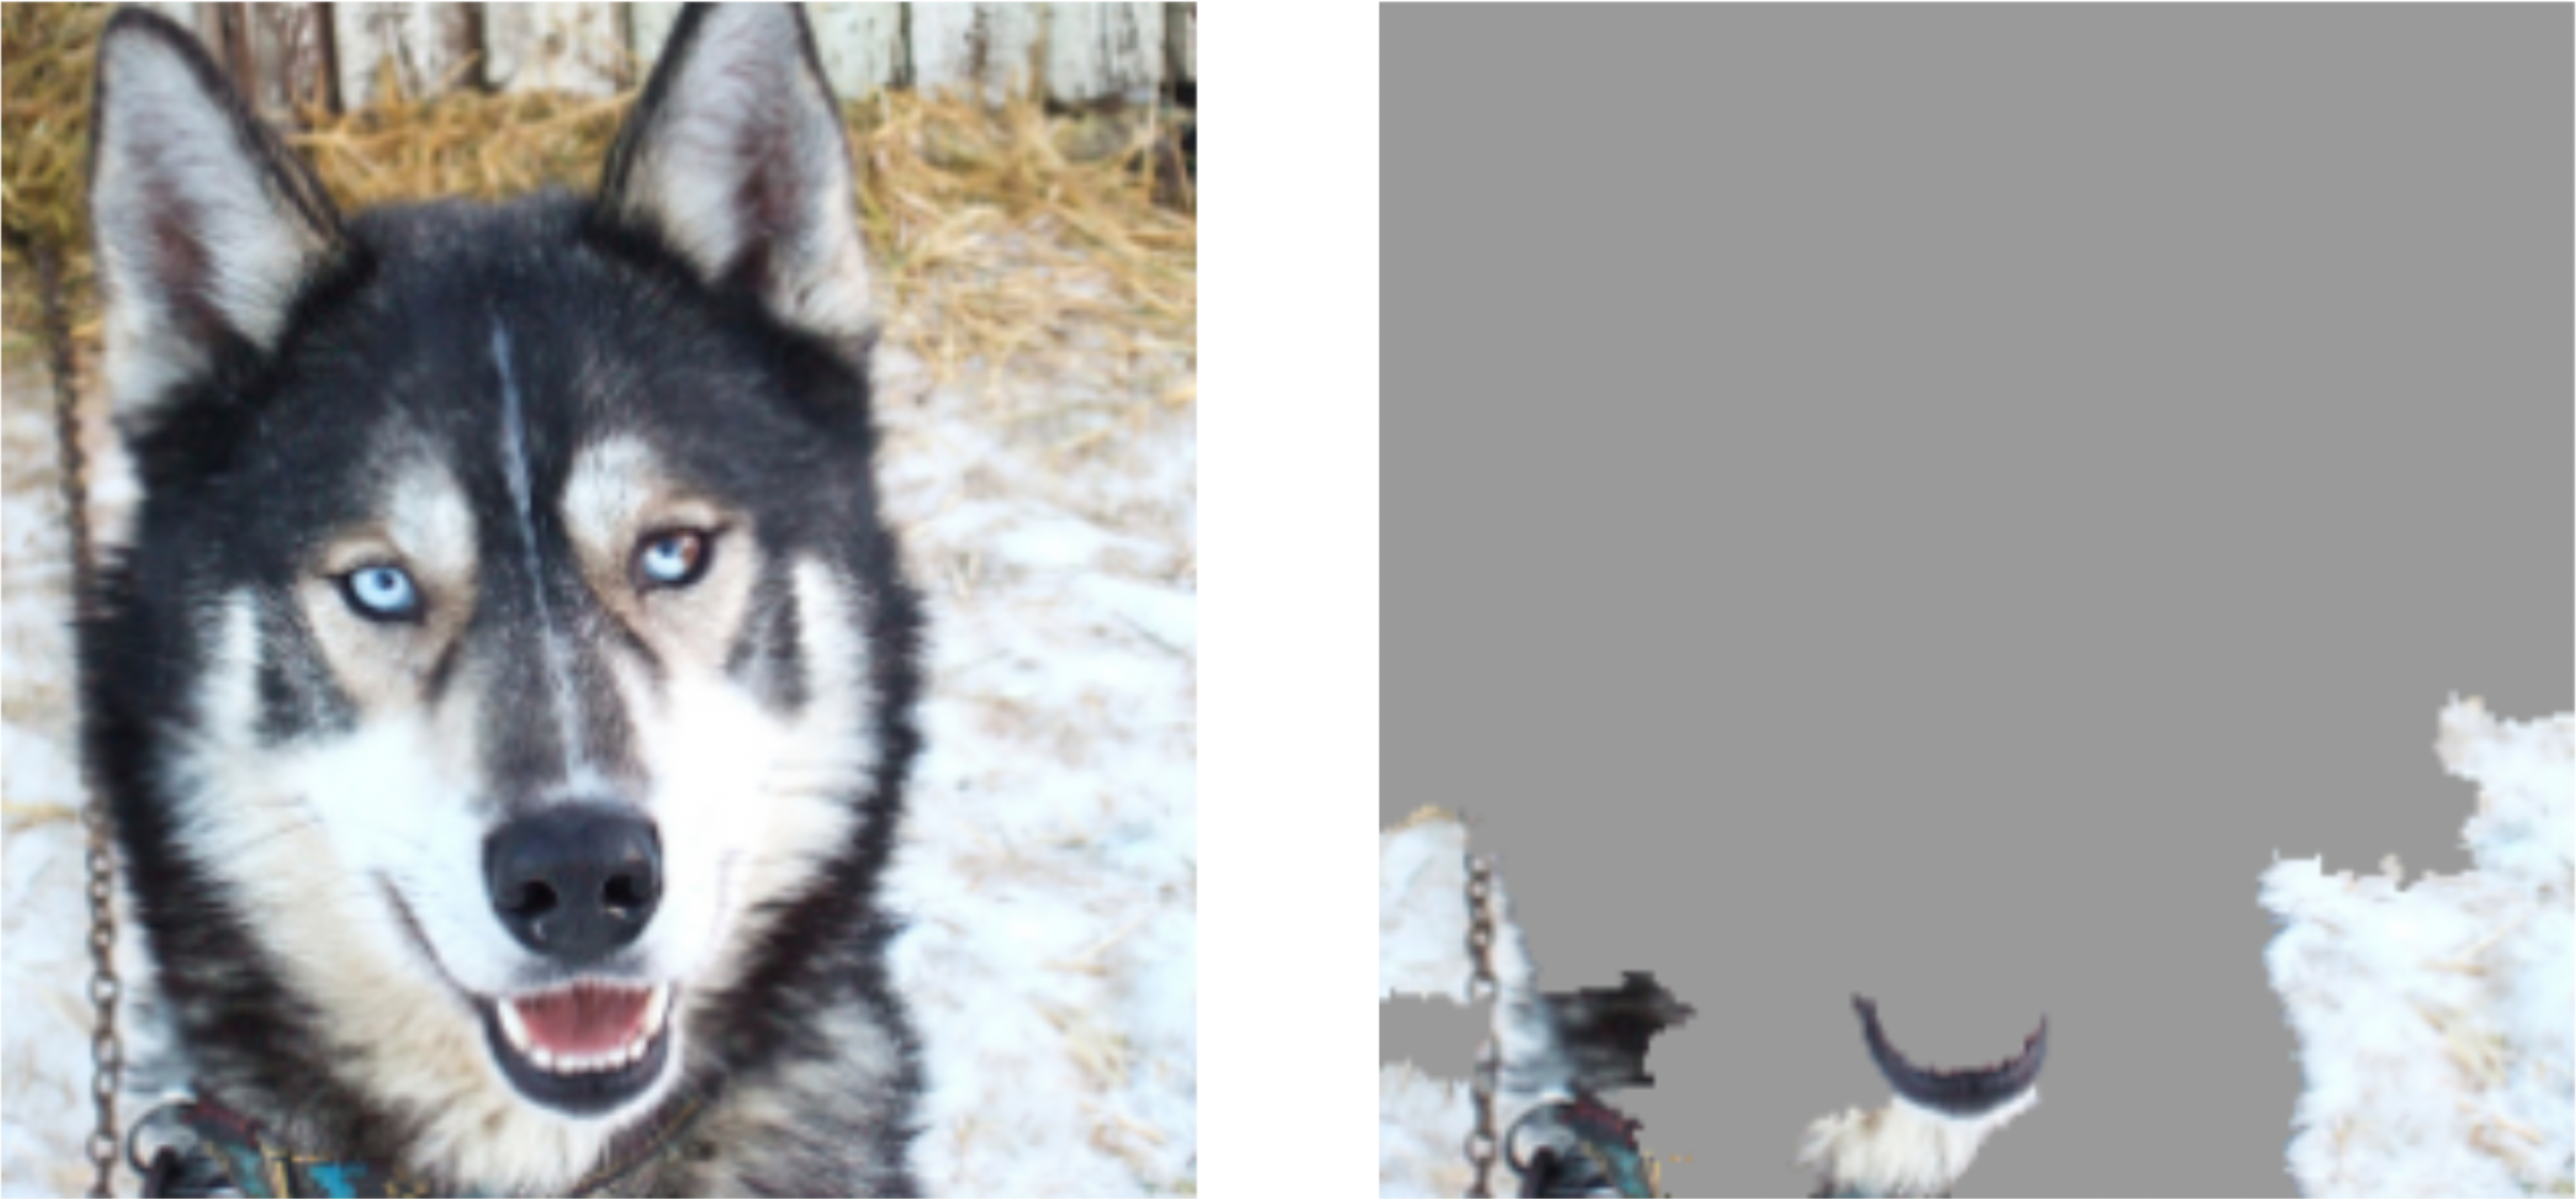
\includegraphics[width=\linewidth]{images/husky_vs_wolf.png}
    \caption[Husky classified as a wolf, alongside an explanation of what the model considered important.]{Husky classified as a wolf, alongside an explanation of what the model considered important. Image by Ribeiro et al. \cite{ribeiroWhyShouldTrust2016}.}
    \label{fig:wolf_husky}
\end{figure} 


% Make humans able to learn from the models
Today's machine learning models are already better than humans in domain-specific tasks, like chess \cite{campbellDeepBlue2002}. Silver et al. \cite{silverGeneralReinforcementLearning2018} proposed the reinforcement learning algorithm AlphaZero, which learns to play chess, shogi (Japanese chess), and Go, only by playing with itself. This method does not get any domain knowledge except the game rules and achieves performance better than humans. Because this algorithm has not seen humans play these games, it does not have human biases and playing flaws in it, and professional game players can learn new moves and techniques by playing with it. 
As performance better than humans is a goal many researchers strive for when it comes to machine learning, it is more important than ever that these algorithms give explanations on what they do and why so that humans can learn new aspects never before thought of, as well as detect flaws that restrict performance, both in humans and machines.

\label{sec:2_background_theory}

\section{Background Theory} % Three pages
% Broader picture
    % NN
    
    % CNN
    

% Image Captioning

    % Image classification


    % Labeling / Captioning


% What is VQA

    % Why is VQA important and interesting
    
    
    % What is the VQA 2.0 dataset




% 
\label{sec:2_related_work}
\section{Related Work} 

In this section, some relevant work for this thesis will be presented. Knowing the main takeaways from these works will help understand the context and assessments that will be made when implementing the methods presented in the next chapter. 
The topics covered in this chapter are computer vision, different methods to create explainable machine learning models, and the development of large language models that lead to the model used in this work.

% Computer vision
% ------------------------------------------
\subsection{Computer Vision}
Computer Vision is the interdisciplinary task of making computers understand and act on visual input. This scientific discipline's main objective is to make computers extract high-dimensional data from the real world using digital images and videos. The extraction of visual information that computers can use includes methods for collecting, processing, analyzing, and understanding the images using statistics, geometry, physics, and learning theory. 

% Object detection
Object detection is a significant part of computer vision that has made astonishing progress. It has been an important research topic because it is one of the fundamental problems in computer vision. Detecting objects form the fundamental basis of other computer vision tasks, such as object tracking, segmentation, and image captioning. Many of these sub-domains' achievements have come from using \gls{cnn} architectures with more layers, trained on larger datasets, and more powerful computers. These main components have made the algorithms capable of learning a deeper understanding of the visual world and learning more fundamental elements of materials, objects, and scenes.  

% Is this relevant?
Krizhevsky et al. introduced AlexNet\cite{krizhevskyImageNetClassificationDeep2017}, as a variant of the \gls{cnn} proposed by LeCun et al.\cite{lecunHandwrittenDigitRecognition1989, lecunGradientbasedLearningApplied1998} seen in Figure \ref{fig:lenet}, both utilizing the backpropagation algorithm \cite{rumelhartLearningRepresentationsBackpropagating1986}
in training. The main difference is that AlexNet uses three more layers, \gls{relu} \cite{fukushimaCognitronSelforganizingMultilayered1975}
, and is running on \glspl{gpu} instead of \glspl{cpu}, which in practice means more efficient use of computing power.
AlexNet achieved impressive results in the ImageNet \cite{dengImageNetLargeScaleHierarchical2009} 2012 Challenge and is often considered the most influential paper published in computer vision. 
Following this paper, there has been an increasing amount of work done and articles published in the domain of deep learning and images during the last decade.

\begin{figure}[htb]
    \centerline{
    \includegraphics[width=1.2\linewidth]{images/LeNet.jpeg}}
    \caption{\gls{cnn} architecture of LeNet-5 proposed by LeCun et al. \cite{lecunGradientbasedLearningApplied1998}.}
    \label{fig:lenet}
\end{figure} 

% XAI
% ------------------------------------------
\subsection{Explainable AI (XAI)}

The rapid growth of artificial intelligence (AI) technologies has led to an increasing demand for transparency and interpretability in machine learning models. While these models have demonstrated impressive performance in various applications, their lack of transparency and interpretability has raised concerns about their reliability, accountability, and potential biases. As a result, the field of explainable AI (XAI) has emerged to address these challenges by developing techniques and tools that enable humans to understand how AI systems work and make decisions.

Explainable AI is an interdisciplinary research field that aims to make AI models more transparent, interpretable, and accountable to human users. It combines techniques from machine learning, human-computer interaction, cognitive science, and other related disciplines to develop methods and tools for explaining the behavior and decisions of AI models. The need for XAI arises from the fact that many machine learning models, especially deep neural networks, are often viewed as black boxes, meaning that their internal workings and decision-making processes are intricate for humans to comprehend. As a result, these models' lack of transparency and interpretability can create distrust among users, limit their adoption, and raise ethical concerns, especially in high-stakes applications such as healthcare, finance, and criminal justice.

An overview of influential methods proposed in \gls{xai} is presented in this subsection.

% LIME
\paragraph{LIME\\}
In pursuing a method that helps the explaining model to be locally faithful to the underlying model, Ribeiro et al. \cite{ribeiroWhyShouldTrust2016} proposed \gls{lime}. This model-agnostic method explains any method by learning an interpretable, less complex model locally around a specific prediction. This approach assures that the explanation is locally accurate and represents the actual inner workings of the model. 
In the same paper, they also introduce a method for explaining the global attributes of the model by framing the task as a submodular optimization problem. The technique is called SP-LIME (Submodular Pick LIME). With this approach, they can achieve global explanations that are locally accurate and faithful to the underlying model in a non-redundant way. LIME will be used later in this thesis as an explanation method adapted to a \gls{llm}.

% SHAP
\paragraph{SHAP\\}
Making non-redundant explanation features faithfully and efficiently is not easy. Lundberg et al. \cite{lundbergUnifiedApproachInterpreting2017} proposed a unified framework for interpreting predictions made by the underlying method. This framework called \gls{shap}, assigns each feature a value of importance for a specific prediction. The framework utilizes the class of additive feature attribution methods and estimates the Shapley % cite
values from cooperative game theory for that prediction. With this approach, they achieve more effective explanations to compute and have better consistency with human intuition than previously proposed methods.  


% Grad-CAM
\paragraph{Grad-CAM\\}
Visually explaining features that contributed to an image prediction can be essential in gaining trust in a model. Selvaraju et al. \cite{selvarajuGradCAMVisualExplanations2020} proposed a technique for making \glspl{cnn} more explainable and transparent by producing visual explanations for the underlying model. The method is called \gls{gradcam}, a generalization of CAM proposed by Zhou et al. \cite{zhouLearningDeepFeatures2016}, and uses the gradients in a single backtrack of any target concept. Therefore it does not need any architectural changes or retraining of the underlying prediction model to produce a localization map highlighting the crucial regions in the image for predicting the given concept, often called a saliency map in computer vision.

% DenseCap


% FLEX
\paragraph{FLEX\\}
While visual-only explanations can give the user insight into which areas of the image were essential in making the decision, they tell little to nothing about why those regions were important. On the other hand, linguistic descriptions give the user an essential understanding of the model's evaluation when predicting. 
Wickramanayake et al. \cite{wickramanayakeFLEXFaithfulLinguistic2019} propose \gls{flex} to merge saliency maps with locally accurate linguistic descriptions. In this approach, they look at the gradients through layers and identify the most critical activations in the single decision. The advantage of looking at different layers is that alongside getting an explanation that is faithful to the underlying model, they also extract features the \gls{cnn} identifies at each layer. A \gls{cnn} may represent high-level concepts, like a "car", at the last layer while identifying features such as texture and color at earlier layers. Using the activations at all essential layers, \gls{lime} achieves an image caption that explains all the essential parts of the prediction using sentences. \gls{flex} maps words to neurons in the \gls{cnn} by looking at high activations of that neuron combined with a word from the caption during the training. For this, they are using a \gls{cnn} and two stacked \gls{lstm} \cite{hochreiterLongShorttermMemory1997} cells.
The \gls{flex} framework is used as a basis for one of the two proposed methods in this thesis. A more detailed description of the specific implementation for this work is discussed later in Chapter \ref{sec3:flex_vqa}.

% VQA dataset
\paragraph{Visual Question and Answering (VQA)\\}
In order to make the linguistic abilities of computers more robust, Agrawal et al. \cite{agrawalVQAVisualQuestion2016} proposed a new dataset called \gls{vqa}. This dataset provides images from the COCO dataset \cite{linMicrosoftCOCOCommon2015}, paired with free-form, open-ended questions and answers corresponding to the content of the images. These questions and answers target different areas of the images, including underlying context and background details. This dataset aims to make models that can learn multi-modal visual and linguistic domain knowledge to get a more general and complete understanding of the world. Models that have done well in this dataset are frequently made up of \glspl{cnn}, to acquire the visual knowledge, combined with an \gls{rnn} % cite
for linguistic understanding.

Even though \gls{vqa} is not strictly \gls{xai}, it is still relevant regarding transparency to the user. \gls{vqa} is an important research area because it provides AI systems with human-readable explanations of their decision-making processes.
By providing a natural language explanation of why a specific answer was generated for a particular question about an image, \gls{vqa} models can help improve \gls{ai} systems' transparency and interpretability. This can be particularly important in domains such as healthcare and finance, where trust and transparency are critical for ensuring that \gls{ai} systems are making reliable and safe decisions. Therefore, it is important to continue developing and improving \gls{vqa} models to provide accurate and interpretable answers to questions regarding images.
Both the methods implemented and investigated in this work will be based on \gls{vqa}, using text to describe the contents of images utilizing different approaches.

\subsection{Large Language Models (LLMs)}

    \glspl{llm} are neural networks with billions or more parameters trained by self-supervised or semi-supervised learning on large amounts of text. They originated around 2018 and have performed competently on a variety of tasks. \glspl{llm} are typically general-purpose models that excel in various roles, with their performance and range of capabilities depending on the number of resources devoted during training. These models demonstrate considerable general knowledge about the world and can learn associations that make the model "memorize" numerous facts and contexts during training. 

    
    
    \glspl{llm} are pre-trained on large text datasets and can be characterized by four parameters: the size of the model, the size of the training dataset, the training cost, and the post-training performance. These variables are related by simple statistical laws called scaling laws. 

    \glspl{llm} serve not only to teach \glspl{ai} human languages but to understand proteins, write software code, and help students. These models are trained with vast amounts of text fed into the AI algorithm through unsupervised learning, allowing the model to find valuable connections in the language. Through this method, a \gls{llm} learns words, their relationships, and the concepts behind them. \glspl{llm} can also be tailored for specific use cases, including through techniques such as fine-tuning or prompt tuning, which feed the model small bits of data that must be focused on to train it for a specific application.
    
    
    However, a disadvantage of \glspl{llm} is that they can suffer from a phenomenon called hallucinations. Generative models can hallucinate because they contain vast amounts of data and organize the information in an unsupervised way. These models tend to make self-confident claims about facts not justified by their training data, which appears plausible but is not factually correct. Because of their size, they can also be challenging and computationally expensive to interpret. An ethical concern about the size of these models is that they are also computationally intensive during training and inference since they are trained on large datasets. As a result, these models have a larger carbon footprint than smaller models. However, there are ways to make these models smaller and faster, which are discussed in this chapter and also provide an overview of the development of large language models.

   

    \paragraph{BERT\\}

    BERT (Bidirectional Encoder Representations from Transformers) is a large-scale neural language model that has made significant contributions to the field of natural language processing (NLP) \cite{devlinBERTPretrainingDeep2019}. BERT is a pre-trained model that uses a transformer-based architecture that has grown in popularity in recent years due to its success in several NLP tasks. Introduced by Google in 2018, BERT is trained on a large corpus of text using an unsupervised learning approach. The model is pre-trained on a task called Masked Language Modeling (MLM), in which a small percentage of the words in a sentence are masked randomly, and the model is trained to predict the original word based on the context of the sentence. This method can be viewed as a "fill in the blanks" task, often called a cloze test, of the training sentences, keeping some words invisible to the model during training and helping the model generalize to new and unseen data. In addition, BERT is trained on an NSP task (Next Sentence Prediction), similar to the GPT models. The model is given pairs of sentences and asked to predict whether the second sentence continues the first.

    The main innovation of BERT is its ability to understand the context and provide contextualized word embeddings. Unlike previous word embeddings, which were static and did not change based on the context of the sentence, BERT can offer different embeddings to the same word depending on its context.
    
    
    
    \paragraph{BART\\}
    Lewis et al. at Facebook presented an \glspl{llm} named BART (Bidirectional and Auto-Regressive Transformer) \cite{lewisBARTDenoisingSequencetoSequence2019}. Like BERT, it uses a transformer-based architecture and is trained on a large corpus of natural language. However, unlike BERT, BART is unique because it integrates a bidirectional and auto-regressive architecture, which makes it well-suited for text generation and summarization tasks. 
    This model is a pre-trained sequence-to-sequence model that can be fine-tuned for various natural language processing tasks. BART is designed to handle auto-regressive, non-auto-regressive, generation, and comprehension tasks. The model is pre-trained on a large corpus of text using a denoising autoencoder objective, which requires the model to reconstruct original text from corrupted versions. Using a denoising autoencoder in pre-training helps reduce hallucinations by training the model to distinguish between real and fake input. 
    The authors demonstrate that BART outperforms several state-of-the-art models on various natural language generation and comprehension tasks, including summarization, question answering, and text classification. They also show that BART can be fine-tuned with relatively little data and can generalize to new domains. 
    However, instead of using Masked Language Modeling and Next Sentence Prediction like BERT, BART is pre-trained using a denoising autoencoder (DAE) objective.

    The DAE objective involves corrupting an input sequence by randomly deleting or swapping tokens and training the model to reconstruct the original sequence. This approach allows BART to handle more complex tasks such as text summarization, sentence generation, and machine translation.
        
    
    
    \paragraph{GPT\\}
    GPT (Generative Pre-trained Transformer) is a set of \glspl{llm} developed by OpenAI \cite{radfordImprovingLanguageUnderstanding2018}. Like BERT and BART, GPT is a transformer-based model but uses only an autoregressive architecture. It is pre-trained on large datasets and tuned for specific tasks. When GPT-2 was released, it was trained on a much larger dataset with significantly more parameters than GPT-1 \cite{radfordLanguageModelsAre2019}. This allowed it to generate more coherent and realistic text than its predecessor. GPT-3 is the third model in the GPT series and was released by OpenAI in 2020. It was trained on an even larger dataset than GPT-2 and had even more parameters, making it one of the largest language models. GPT-3 could generate even more readable and human-like text than its predecessors and perform various NLP tasks without explicit training \cite{brownLanguageModelsAre2020}. At the time of writing, the last published GPT model was GPT-4, which is still an autoregressive model but also includes multimodality \cite{openaiGPT4TechnicalReport2023} by making it able to interpret images. To reduce the effects of hallucinations on a generated output, GPT implements a combination of methods such as filtering and sampling.
    
    These models have proven to be versatile and powerful tools for NLP. GPT models have significantly influenced the NLP field, and many researchers and developers have used it as a starting point for their projects. Fine-tuned chatbot versions of GPT-3 and GPT-4 have been made available for public interaction under the name ChatGPT \cite{ChatGPT}.

    
    
    
    
    % LLaMA
    \paragraph{LLaMA\\}
    The \gls{ai} department of Meta, previously Facebook, released a modified architecture for a \gls{llm} called \gls{llama} \cite{touvronLLaMAOpenEfficient2023}.
    %This model with corresponding weights was not released to the public, but after a leak, \cite{vincentMetaPowerfulAI2023}, both the model and its weights became available to the public. 
    These models are created to compare to other \glspl{llm}, such as GPT-3 \cite{brownLanguageModelsAre2020}, Chinchilla \cite{hoffmannTrainingComputeOptimalLarge2022}, or PaLM \cite{chowdheryPaLMScalingLanguage2022}, while keeping the number of parameters considerably smaller. In the paper where Hoffman et al. propose the Chinchilla model, they also present insight into how models scale the best in conjunction with the size of the available dataset. The authors of \gls{llama} use this insight to make the model with fewer parameters perform well by training it on more tokens. The dataset that the \gls{llama} model is pre-trained on is publicly available and disclosed, which makes it compatible with open-source. The architecture is based on the transformer \cite{vaswaniAttentionAllYou2017}, with various improvements inspired by other \glspl{llm}. Some of these improvements are pre-normalization, inspired by GPT-3 \cite{brownLanguageModelsAre2020}, which improves the training stability by normalizing the input of each transformer sub-layer instead of the output. Like the PaLM model, they also use a SwiGLU as the activation function, first introduced by Shazeer at Google \cite{shazeerGLUVariantsImprove2020}, instead of \gls{relu}. Shazeer showed it to improve the perplexities of transformer-based models. To make the self-attention mechanisms in the transformer position-agnostic, the authors implement a method called Rotary Position Embedding (RoPE) introduced by Su et al. This method allows both flexibilities of sequence length and faster convergence in fine-tuning compared to normal self-attention. With the 13 billion parameter version of \gls{llama}, the authors show that this model outperforms the GPT-3, with 175 billion parameters, on several evaluation metrics. Because the \gls{llama} model is ten times smaller than GPT-3, it can also be run on a single \gls{gpu}. These steps towards smaller, capable models benefit both the carbon footprint and inference compute budget and permit democratizing \glspl{llm} by making a model that can run on consumer hardware.

    \paragraph{Alpaca\\}
    The work in this thesis uses this Alpaca model to interpret images. More of how this model is implemented is discussed later in Chapter \ref{sec3:alpaca_vqa}.
    
    With Taori et al., Stanford University released an open-source fork of this \gls{llama} model, with some modifications, called Alpaca \cite{taoriStanfordCRFM, taoriStanfordAlpacaInstructionfollowing2023}. The Alpaca model is a fine-tuned model, with a 7B \gls{llama} model as the base model, trained on 52 thousand instruction-following tasks generated by OpenAI's text-DaVinci-003 model \cite{OpenAIAPI} using techniques from the Self-Instruct paper proposed by Wang et al. \cite{wangSelfInstructAligningLanguage2022}. Figure \ref{fig:alpaca_training} shows an overview of the Alpaca training procedure and how the dataset was built. By using text-DaVinci-003 to generate instructions, the team was able to train the model and generate the dataset for a significant cost reduction compared to traditional methods, totaling only \$600, with \$500 using OpenAI API to create the dataset and \$100 to rent 3 hours on 8 Nvidia 80GB A100 GPU cards. Reducing the cost of training an \gls{llm}, comparable to models much more expensive to develop, helps democratize these models and make them available to more people for less cost and energy.

    
    To address the ethical issue of not knowing whether a text is generated by an \gls{ai}, the team also implemented the method proposed by Kirchenbauer et al. \cite{kirchenbauerWatermarkLargeLanguage2023}. This method embeds "green" or marked tokens into the generated text, which are invisible to humans but can be detected by an algorithm analyzing a short span of these tokens.  
    The authors argue that the watermark can be embedded with negligible impact on text quality and can be detected with an efficient open-source algorithm without access to the language model API or parameters. The watermark works by choosing a random set of green tokens before generating a word and using a soft watermarking rule to encourage the input of green tokens during sampling. The authors propose a statistical test to detect the watermark with interpretable p-values and derive an information-theoretic framework to analyze the sensitivity of the watermark.

    Given the need for less computational resources, leading to a reduced carbon footprint, and the ability to disclose the generated text as computer-generated, the Alpaca model represents a favorably ethical and transparent option for users of a system compared to other \gls{llm}. As such, it is an appropriate choice as a starting point for this thesis. This model has many of the benefits that \glspl{llm} can provide, like knowledge of vasts amount of data, while still being able to customize it to a specific task through fine-tuning. This process enables the model to adapt to a particular assignment while retaining the knowledge acquired from its initial training data.

    
    % Data flow
    \begin{figure}[htb]
        \centerline{
        \includegraphics[width=17cm]{images/alpaca_framework.jpeg}}
        \caption[Overview of the Stanford Alpaca training procedure.]{Overview of the Stanford Alpaca training procedure.\\Figure by Taori et al. \cite{taoriStanfordCRFM}}
        \label{fig:alpaca_training}
    \end{figure}
\section{Summary}
\label{sec:2_summary}

\begin{comment}
SUMMARY: Often, we recommend ending this chapter (and all chapters after except the conclusion) with a summary section. The aim is to give an overview of, and tea-spoon-feeding the reader with, what he/she should have learned reading this chapter. What can be concluded from this chapter? 
How does the information given here give arguments for your problem statement? Finally, lead to the next chapter (“... and we will therefore in the next chapter address these challenges, and describe our ideas/implementation/...”)
\end{comment}


This chapter provides an overview of the background and motivation for using the concept of \gls{xai} in various applications. 
The discussion focuses on the challenge of understanding decision-making processes in complex AI systems and the necessity for more transparent machine learning models, particularly in applications where the consequences of erroneous decisions can be severe. 


The chapter also delves into the history of AI and its two main paradigms: symbolic and connectionist AI. 
Moreover, it lays out various machine learning techniques, including supervised, unsupervised, and semi-supervised learning, as well as deep learning and neural networks.


The key takeaways from this chapter are:

\begin{itemize}
    \item The importance of XAI in building transparent and trustworthy AI systems for real-world applications.
    \item The diverse techniques used in machine learning, why they are used, and how they differ.
\end{itemize}

The topics discussed in this chapter provide insight into the importance of designing systems transparently. An understanding of the data and models used helps researchers build better and more appropriate systems, and users can better understand why those systems predict what they do.

\begin{comment}
    How does the information given here give arguments for your problem statement?
\end{comment}

This work will use a combination of a \gls{cnn}, an \gls{llm}, and \gls{xai} to conduct its experiments. 
These experiments will investigate further how these methods can be understood and explained. 


The following chapter will therefore introduce some methods that address some of the challenges presented in this chapter. Two different approaches are presented, and both have multimodal capabilities. Both models are based on the \gls{vqa} task, where one model uses a traditional \gls{vqa} architecture, with an explanation method that explains visual features using text. The other model also describes images using text but is based on an \gls{llm}. 
The next chapter is, therefore, a summary of methods used to answer the research goals of this thesis.

\chapter{Methodology}
\label{sec:3_methodology}

\begin{comment}
This chapter may have many names. Lately, many have named it "Methodology", but names like "Design and Implementation", a "name" of a developed system, etc. are also often used. Just find a name that matches your research. Regardless, the important thing here is to describe YOUR research.

INTRO: Again, start the chapter with a sentence or two explaining why you have this chapter (repeating the last sentences from the proposed summary in the previous chapter) - assuming that some readers have not read the previous chapter.

MIDDLE SECTIONS: What are your ideas? Your solutions. How have you done "things"? Implementation details. Frameworks used. Etc. Also, discuss alternative ways of doing things and explain why you have chosen to do things as you have. WHAT! HOW! WHY!

SUMMARY: End this chapter with a summary section. Summarize what you have done and why! Main knowledge gained. What have we learned? Lead to the next chapter, stating that you will test your prototype.
\end{comment}


% INTRO:
% Again, start the chapter with a sentence or two explaining why you have this chapter (repeating the last sentences from the proposed summary in the previous chapter) - assuming that some readers have not read the previous chapter.


%This chapter will introduce some methods that address some of the challenges presented in this chapter. 
In this chapter, the two methods proposed in this work are presented in more detail. The overall goal of these two methods is to explore how different machine learning models can implement explanatory methods in various domains that still provide value to the user. Different model architectures represent data in different ways. 
This chapter highlights how insights into these representations can give a researcher or user a new understanding of the data and models used.
Both models presented in this chapter have multimodal capabilities, specifically in visual and linguistics. The way they achieve this multimodality differs. 

The first model uses a classical \gls{vqa} architecture, with the addition of the \gls{flex} framework. 
Using this framework, the model can label feature maps in the \gls{cnn} to get information from the visual domain translated into natural language. The explanation originates, therefore, from the visual domain, translated into text. 


The second method introduces a large language model (LLM) combined with a standard \gls{cnn}. The image features of the \gls{cnn} get translated into text, and the explanation happens in the text domain. 

Therefore, these two models discussed in this chapter will investigate explanations originating from different domains.

%The other model also describes images using text but is based on a large language model. The next chapter is, therefore, a summary of methods used to answer the research goals of this thesis.

% MIDDLE SECTIONS:
    % Implementation
    \section{FLEX-VQA}

    This section will delve deeper into implementing the first proposed method, FLEX-VQA. The name originates from the framework FLEX, originally introduced by Wickramanayake et al. \cite{wickramanayakeFLEXFaithfulLinguistic2019}, combined with visual question and answering (VQA). 
    
    \label{sec3:flex_vqa}
        \subsection{Overview}
        % What:

        % FLEX
        To make \gls{vqa} models easier to understand for the user, the explanation can originate from either of the two modalities of the model, either the language model, the image model, or both. 
        The method presented in this experiment will address this task using the cross-modality explanation method \gls{flex}. An overview of the \gls{flex} model has already been described shortly in sub-chapter \ref{sec:2_related_work} on page \pageref{sec:2_related_work}. This method is relevant to this method because it explains the network's visual reasoning of why a picture should be in a given class using natural language. The \gls{flex} framework combines a \gls{cnn}, which is pretrained on the specific task and does not need any further training that alters the \gls{cnn} to give it explainable abilities. An overview of the original \gls{flex} framework can be seen in Figure \ref{fig:flex_overview}.

        \begin{figure}[htb]
            \centering
            \centerline{
            \includegraphics[width=17cm]{images/FLEX_overview.png}}
            \caption[Overview of the FLEX Framework.]{Overview of the FLEX Framework.\\
            Figure credit: Wickramanayake et al. \cite{wickramanayakeFLEXFaithfulLinguistic2019}.}
            \label{fig:flex_overview}
        \end{figure}

        \subsection{The motivation for this method}

        % Why:
        By using \gls{flex} as a starting point, the purpose of the method in this experiment is to adapt it to have \gls{vqa} abilities. In order to make this adaption, the dataflow shown in Figure \ref{fig:architecture_proposal} is proposed. Using this technique, a user can get an answer for a question regarding an input image that is both in natural language and faithful to the underlying \gls{cnn} model, making it more explainable and transparent. The explanation is faithful to the underlying model since it uses the actual gradients in the \gls{cnn} to find the words used to answer the question. 
        This feature ensures that if the underlying \gls{cnn} model has learned features that correlate with the answer but are not the intended or logical features to pay attention to, these flaws get communicated to the user. Making a model that can explain what it considers important to a user, also when flawed, is important when making a system where a user can make a factually based decision in trusting the answer.
        

        % More in detail on how FLEX works. 
        \subsection{Original FLEX in more detail}
        \label{sec3:flex_detailed}
        First, the \gls{flex} framework works by having a \gls{cnn} predict the class of an input image. Given the image and its predicted class $c$, the method finds a subset of the most important feature maps from each layer in the pretrained \gls{cnn}. To find the global activation score of each feature map, it sums up each neuron in the layer and then repeats this process for each layer in the \gls{cnn}. After that, it sorts the layers in order of importance and chooses a subset of $n$ layers so that the subgroup has a combined importance over a predefined threshold. When a subset of the most important visual features is collected, \gls{flex} connects these visual features with linguistic features. 

        \gls{flex} uses the \gls{gradcam} technique proposed by Selvaraju et al. \cite{selvarajuGradCAMVisualExplanations2020} to do a backward pass through the feature maps of the \gls{cnn} to find the largest class activation maps when predicting a class. This information is then used to map words to important visual feature extractions in the network. This mapping of words combines the separable feature layers salient layers of the \gls{gradcam} method with natural language to make better explanations.
        
        The way \gls{flex} archives explainability is to find a connection score between a word ($w$) to the elements of the important feature maps ($F$) so that the word ($w$) best describes the important visual element ($v$) in each feature map. With a given natural language description of the ground truth ($D_I$) of an image ($I$), \gls{flex} uses the corresponding description for every image and builds a dictionary that contains all words in every description seen in the training data. This dictionary ($D$) is used when describing new images during testing. 
        Creating this combined dictionary is conceptually similar to how language models generate a dictionary of tokens used for tokenization.
        For each word ($w$) \gls{flex} calculates the co-occurrence score for each feature ($v \in F$), using the Dice score \cite{diceMeasuresAmountEcologic1945, sorensenMethodEstablishingGroups1948}, as seen in Equation \ref{eq:dice_score_flex}. The word with the highest co-occurrence score gets associated with the visual feature ($v$). 
        
        \begin{equation}
            \textit{score}(w, v) = \frac{2 \times \textit{occur}(w, v)}{\textit{count}(w) + \textit{count}(v)}
        \label{eq:dice_score_flex}
        \end{equation}

        When the dictionary $D_I$ for each image and the dictionary for all images $D$ is computed, the dictionary for the individual class labels can be found. This class label dictionary ($D_c$) contains the combined dictionary of each image of a specific class and can be defined as $D_c = \bigcup D_I$, where the class label of $I$ is $c$. 
        Lastly, the dictionary $D_r$ is the words extracted recursively from the \gls{cnn}. When an image is inputted, and the class is predicted, \gls{flex} starts at the last convolution layer and finds the top-$k$ features from that layer and their associated words. This collection of associated words from feature maps is done recursively until the first convolutional layer is reached, and the union of all these words is named $D_r$.


        To describe decision-relevant features, \gls{flex} computes the relevance of a word $w$ to each of the dictionaries using the formula in Equation \ref{eq:relevance_calculation_flex}, where $D_x$ is a placeholder for $D_r$, $D_I$, and $D_c$.

        \begin{equation}
            \operatorname{relevance}\left(w, D_x\right)=\left\{\begin{array}{cl}
            0 & w \notin D_x \\
            -\log \left(\frac{\left|D_x\right|}{|D|}\right) & \text { otherwise }
            \end{array}\right.
            \label{eq:relevance_calculation_flex}
        \end{equation}

        When the relevance scores for each dictionary are calculated, the relevance vector $z$ is defined as in Equation \ref{eq:relevance_vector_flex}:

        \begin{equation}
            z = (g(w1), g(w2), ..., g(w\left|D\right|))
        \label{eq:relevance_vector_flex}
        \end{equation}

        Where $w_i$ is the $i^{th}$ word in $D$ and
        \begin{equation*}
            g(w_i) = relevance(w_i, D_r) + relevance(w_i, D_I ) + relevance(w_i, D_c)
        \end{equation*}
  

        To train the framework to generate a textual description, \gls{flex} uses two stacked LSTMs, where the first LSTM receives the ground truth word $w_{t-1}$. The second LSTM gets the hidden state of the first LSTM, concatenated with the visual feature vector from the \gls{cnn}. The output of the second LSTM is encoded to vocabulary space to produce a conditional probability distribution, defined as:

        \begin{equation}
            P (w_{t-1} | w_{\le t-1}, I)
        \label{eq:flex_contitional_proba_func}
        \end{equation}
        
        This distribution samples the current word $w_t$ at time step $t$.  
        The relevance vector $z$ is element-wise multiplied by this probability distribution to produce the relevance loss and is defined as:

        \begin{equation}
            \operatorname{loss}\left(w_t, I\right)=\max \left(\boldsymbol{z} \odot P\left(w_t \mid w_{\leq t-1}, I\right)\right)
        \end{equation}

        When no ground truth label is available during interference, \gls{flex} samples from the conditional distribution in Equation \ref{eq:flex_contitional_proba_func} to get the next word then passed as the input to the LSTM in the next step.
                

   
        This labeling of visual features can be reminiscent of DenseCap proposed by Johnson et al. \cite{johnsonDenseCapFullyConvolutional2016}, and Neural Baby Talk proposed by Lu et al. \cite{luNeuralBabyTalk2018}. The main difference between these methods and \gls{flex} is that \gls{flex} can be added to a network after the architecture is finalized, trained, and evaluated. In theory, the framework is agnostic to the underlying network. However, one limitation is that the visual encoder must have a property in which distinct parts of the image activate distinct parts of the network. 
        
        
        

        \subsection{Implementation}
        % How:
        Given that \gls{flex} can combine information from the visual domain with natural language, it is an exciting framework to explore in the field of \gls{xai} and \gls{vqa}. A modified architecture to \gls{flex} is presented in this thesis, as seen in Figure \ref{fig:architecture_proposal}. This proposed architecture has unfortunately not been tested because of technical hindrances outside the scope of this work. A more detailed explanation of these hurdles is described in subsection \ref{subsec:no_flex}. However, since much of the available time for this thesis was spent researching this approach and solving the hurdles, an overview of the architecture will still be proposed in this section.


        % Dataset: VQA 1.0 vs. 2.0
        \subsubsection{Dataset: VQA 1.0 and COCO}
        The dataset chosen for this experiment is the VQA 1.0 dataset \cite{agrawalVQAVisualQuestion2016} instead of the more balanced VQA 2.0 \cite{goyalMakingVQAMatter2017}. 
        This experiment's goal is not to achieve state-of-art accuracy but to test the validity of this method. The VQA 1.0 dataset allows the \gls{vqa} model to learn biases in the data that will be utilized in this method. Because of its unbalance, the authors of the VQA 1.0 dataset propose to use a k-way classification with 1000 classes. The rationale behind this decision is that the top thousand classes cover 82.67\% of all the train and validation answers. Optimizing this way makes the assignment no longer open-ended but a more straightforward task by choosing one class out of a thousand. 
        
        This optimization will make the answer easier to compute, reducing training time and making it easier to control if the prediction is correct. Another benefit of this simplification is that the FLEX-VQA method can use the answer as a class, making it more efficient to adapt it to the \gls{flex} framework. This is because the \gls{flex} method builds a dictionary for each class ($D_c$). 
        In order to make the dictionary $D_c$, the method will need descriptions for each image. 
        Another benefit of using the VQA dataset is that the images originate from the Common Object in Context (COCO) dataset \cite{linMicrosoftCOCOCommon2015}. This dataset is a large-scale object detection, segmentation, and captioning dataset, meaning that the images in the VQA dataset are already described in COCO. 
       

        % Input from essay here.
        \subsubsection{Proposed architecture}
        \label{sec3:proposed_architecture}
        
        Figure \ref{fig:architecture_proposal} shows how the data flow in the proposed method is supposed to work. It closely follows the original \gls{flex} architecture, with adaptations to make it answer questions. It consists of a \gls{cnn} that extracts visual information and a 2-layered \gls{lstm} \cite{hochreiterLongShorttermMemory1997} \gls{rnn} that combine linguistic information with extracted visual features. 
        The \gls{cnn} used in this implementation is the same as in the original framework, which is a modified VGG-16. The modification is a technique proposed by \cite{gaoCompactBilinearPooling2016} et al. called Compact Bilinear Pooling, which reduces feature dimensionality without sacrificing performance. This ensures a more efficient and faster training and inference time, which also has the potential benefit of reducing the risk of overfitting.


        
        
        % Explain the proposed data flow/architecture 
        % VQA
        
        The wanted requirements of the system will need to be defined before any method can be developed. 
        The method should be able to have an image as input alongside a question related to the content of this image. The wanted output is a locally accurate answer to the question and a description that is also locally accurate to the model. 
        
        \textbf{\\The VQA model\\} 
        As shown in Figure \ref{}, an architecture can be utilized to make a model that achieves the required features. This figure shows in more technical detail the architecture in Figure \ref{fig:architecture_proposal}. This technical figure consists of a standard \gls{vqa} model with a k-way classification optimization. This architecture is essentially the same as the one presented in the original VQA 1.0 paper, called \textit{deeper LSTM Q + norm I}, which achieves an accuracy of 57,75\% on the complete test set. 
        This network comprises an image pipeline (\textit{norm I}) with activations from the \gls{cnn} being $l_2$ normalized. The question pipeline (\textit{deeper LSTM Q}) consists of an \gls{lstm} with two stacked layers. 
        The image embeddings are then transformed to a dimensionality to match the question embeddings. This is done by a fully-connected layer, which makes the image features a vector with a length of 1024.

        When the image and question features have the exact dimensions, they are merged by pointwise multiplication. 
        This fusion vector is then passed through a fully connected neural network with two hidden layers, 1000 hidden units in each layer, and a dropout of 0.5.
        Finally, the answer with the best fit is found by passing the result of the  fusion vector through a SoftMax layer to predict the final class.
        
        
        
        
        

        % FLEX
        \textbf{\\FLEX\\}
        Since the \gls{vqa} system is now a classification task, it can be matched with the \gls{flex} framework. 
        The importance score is recursively calculated using the image features in each feature map of the \gls{cnn}. The formula used in this calculation is shown in Equation \ref{eq:flex_activaiton_score}, where $Z$ is the total number of neurons in the feature map $A$, the predicted label for class $c$ is $y^c$ and $a_{ij}$ is the $ij^{th}$ neuron in $A$.

        \begin{equation}
            \alpha^c = \frac{1}{Z} \sum_i \sum_j \frac{\partial y^c}{\partial a_{ij}} 
        \label{eq:flex_activaiton_score}
        \end{equation}


        In order to remove negative influence and only evaluate scores contributing to the specific class, the importance scores $\alpha^c$ are then multiplied with a \gls{relu}. These positive-only activation scores are then fed into the secondary stacked LSTM of the \gls{flex} framework, which also gets the hidden state from the first LSTM. This stacked LSTM network is separate from the LSTMs of the \gls{vqa} system, as it is trained only to output descriptions, whereas the one in the \gls{vqa} is used to encode the question features. 
        The rest of the \gls{flex} framework is the same as described in Section \ref{sec3:flex_detailed}, as the main difference between the original \gls{flex} and this method is that instead of the \gls{cnn} predicting a class, the classification method now predicts an answer using the \gls{vqa} model.
        
        
        
        % Training
        \textbf{\\Training and testing\\}
        Given that \gls{flex} is a post-hoc explanation method, it does not need to be trained simultaneously as the \gls{vqa} system. This separation ensures that the \gls{vqa} system can be trained separately from the explanation system and, thereby, can be tuned to achieve satisfactory accuracy before the explanation system is introduced.
        However, even though the systems are separate, the explanations are still connected directly from the extracted image features and, therefore, will be locally accurate to the \gls{cnn} method.

        % Train VQA
        In order to train the \gls{vqa} system, the input image with corresponding questions and their ground truth answers is supplied. The VQA 1.0 dataset contains all these image-question-answer pairs and will be used in this experiment.
        Then entire \gls{vqa} model is trained end-to-end using a cross-entropy loss, as described in the VQA 1.0 paper, where it was presented originally.

        % Train FLEX
        The \gls{flex} is a separate model that is outside of the \gls{vqa} model and, therefore, will need to be trained after the implemented \gls{vqa} method is fully trained. Some optimizations can still be implemented to make this training process faster. The optimization, with a considerable impact on training time, is to precompute the image features when the \gls{vqa} system is trained. Because \gls{flex} uses the image features for each image together with the predicted answer, these can be saved during \gls{vqa} training so that they do not need to be fed through the \gls{vqa} model once more.


        To train the \gls{flex} framework to the task at hand, it must have extracted image importance scores, a ground truth description of the image from the COCO dataset, and the predicted answer for the question. 
        The answer is, in this experiment, regarded as the class label and, therefore, needed when \gls{flex} makes the dictionary $D_c$. The dictionary $D_I$ contains the image description, and the relevance dictionary $D_r$ is calculated using the importance scores from the \gls{cnn}.

        While testing the combined system, the \gls{vqa} method still needs an image and related questions. Then the predicted answer is made by the fully connected network. This answer defines the class dictionary $D_c$ that the \gls{flex} framework uses when making a conditional probability distribution. This distribution contains the combined relevance defined by $z$, which is a function of the relevance for $D_c$, $D_I$, and $D_r$, as described in Equation \ref{eq:relevance_vector_flex} in Section \ref{sec3:flex_detailed}.

        The \glspl{lstm} gets trained by feeding each word in the ground truth caption into the first layer alongside the hidden state of the \gls{lstm}. This is used to compute the next state, which gets concatenated with relevant activation scores from the \gls{cnn} and is input to the second and last, \gls{lstm}-layer. 
        The output from the second \gls{lstm}-layer is encoded to vocabulary space to make a conditional probability distribution that will later be used to calculate the probability of predicting that word, given the given image features. The word with the highest probability is chosen and used as input in the first layer of the LSTM.
        This word prediction is repeated until the stop word is predicted. 
        


    
            
        \begin{comment}
            During the training of the method proposed in this thesis, an image and its corresponding questions and answers from the \gls{vqa} dataset are used as input. The images are fed through a \gls{cnn}-network, which can be pretrained on a larger dataset, such as ImageNet \cite{dengImageNetLargeScaleHierarchical2009}. This is because the explaining method utilizes feature maps in each layer of the \gls{cnn}, so it is agnostic on what type of \gls{cnn} it is and what dataset it is trained on earlier. The \gls{cnn} predicts a class of what it sees in the image and, with a backward pass, finds important feature maps in each  convolutional layer. Each feature in the set of important feature maps gets associated with a word and stored in a relevance vector. This process is done by computing a co-occurrence score between each word in the ground truth caption and the feature. The feature with the highest co-occurrence score gets linked with that feature. 
        
                % LSTM
             
            
                % Testing
            The architecture takes an image and an optional question as input during prediction. The \gls{cnn} extracts important features in the layers, which get fed into the \gls{lstm}. 
            
            If no question is input to the algorithm during prediction, the model will use the most accurate predicted answer caption that describes the image as a whole as a caption for the image. On the other hand, if a question is submitted alongside the image, the \gls{lstm} will generate captions that answer the question asked and then chose the most decision-relevant answer as the caption. 
        \end{comment}
        
        
        
        
        % Data flow
        \begin{figure}[htb]
            \centering
            
            \includegraphics[width=\linewidth]{images/architecture_proposal.png}
            \caption{Proposal of the data flow and components explored in this experiment.
            %Figure by the author.
            }
            \label{fig:architecture_proposal}
        \end{figure}
                
                
        

        
        
        \begin{comment}
            Neither the \gls{cnn} nor the \glspl{lstm} needs to be specifically trained to be explainable. 
            The architecture uses the underlying nature of the models to build a transparent answer to the underlying model and explains to the user what the model values as important. 
    
            
            However, in order to make the method work for a specific case, the \gls{cnn} has to be trained or fine-tuned to the specific dataset. This is because \gls{flex} uses the predicted class to build a dictionary of words for each class. 
        
            If the specific dataset has few images available for training, it can be pre-trained on a larger dataset, like ImageNet, and fine-tuned to the specific dataset. By using this pre-training, the \gls{cnn} can benefit from transfer learning so that general concepts and features can be learned from a general dataset, and valuable data samples for the specific task can learn the fine-grained features specific to this task.
    
            The original \gls{flex} framework uses the LSTMs to generate descriptions based on associated words from activated neurons. In order to make this framework accept question-answer pairs, the LSTMs are trained on questions and ground-truth pairs instead of descriptions. The theory is that a system trained on this question-answer (QA) pairs will still provide the model with an understanding of the objects in images to make a description. 
            For this theory to work, the QA pairs will need to be structured so that the model can learn about objects, locations of objects, time of actions, who is doing the action, why the action is performed, and how the action is performed. An example of a dataset that fulfills these descriptions is the Visual7W dataset, introduced by Zhu et al. \cite{zhuVisual7WGroundedQuestion2016}. 
        \end{comment}
        
        



        \subsection{Why this method has no experiments}
        \label{subsec:no_flex}

            % Intro
            To implement the proposed architecture as shown in figure \ref{fig:architecture_proposal}, it was natural to use the original code from the \gls{flex} paper as a starting point.
            The authors of the \gls{flex} paper also released the code used to do the experiments in the article on GitHub\footnote{https://github.com/sandareka/FLEX} to encourage others to iterate on their method. The original experiments use a \gls{cnn} called Compact-Bilinear Pooling, a classifier proposed by Gao et al. \cite{gaoCompactBilinearPooling2016}. While the FLEX framework is designed to be model agnostic, the actual implementation of the experiments is tied closely with the \gls{cnn}, which proved to be a hurdle when trying to recreate the results in the paper and expand on the architecture and features. 
            This method mainly does not provide finished experiments or results because an outdated machine learning framework makes compact-bilinear pooling \gls{cnn} practically impossible to execute. 
            Combined with the tight integration between the implemented \gls{flex} method and the \gls{cnn} method, considerable resources have been put into separating these two methods, customizing the software, and building containers around it, with no success.
    
            
            \paragraph{The original implementation of FLEX\\}
            For \gls{flex} to work, it needs to get important features from the \gls{cnn}. This is an essential part of the framework and therefore needs insight into how the layers of the \gls{cnn} are structured.
            The implemented version of the original \gls{flex} architecture uses the Compact-Bilinear Pooling \gls{cnn}, which in short, uses kernelization to reduce the number of dimensions of bilinear features to make it more computationally efficient at the cost of having an architecture that deviates somewhat from a more traditional \gls{cnn} architecture. Therefore, the authors of the \gls{flex} paper have implemented a version of the framework that addresses these special considerations when calculating co-occurrence metrics between words and features. 
        

            \paragraph{Why Caffe was needed\\}
            % Why Caffe was needed
            To use the same \gls{cnn} as the original \gls{flex} in a new context, as in this experiment, would require retraining or fine-tuning this network to suit the images in the given dataset. This would require the Compact-Bilinear Pooling model to train using the new pictures in the specific dataset. Alternatively, a new \gls{cnn} could be chosen that could be merged with the \gls{flex} framework. The original Compact-Bilinear Pooling came with pretrained weights from training on the Caltech-UCSD Birds (CUB) \cite{PeronaLabCUB2002011} dataset. This dataset has images from Flickr and ImageNet containing a subset solely focused on bird species and a relatively small amount of photos (11,788, compared to 14 million images in ImageNet \cite{dengImageNetLargeScaleHierarchical2009}). Therefore, the original weights are best fit to classify this CUB dataset and will require retraining outside this specific task.
            Because of how the original \gls{flex} framework is structured, it would need to be substantially rewritten for a new \gls{cnn} to be used in place of the Compact-Bilinear Pooling. Therefore the best way forward was to use this \gls{cnn}, like the original method.

            \paragraph{Getting Caffe to run\\}
            % Getting Caffe to run
            To train the Compact-Bilinear Pooling on a new dataset, the underlying machine learning framework it was built in had to be installed.
            This framework is named Caffe and is a deep learning framework developed by Berkeley AI Research (BAIR) / The Berkeley Vision and Learning Center (BVLC). It's a precursor to the framework  Caffe2, which was initially built by Facebook and is now merged with PyTorch. Because Caffe was forked into Caffe2, the development of the original stagnated. Developers implemented new features and compatibility in Caffe2, while the original Caffe has not received an update since 2017. 
            Because of the rapidly evolving nature of software and hardware since 2017, it proved to be a nontrivial task to get Compact-Bilinear Pooling written in Caffe to run on the hardware available during this project.
            The \gls{flex} framework is implemented in TensorFlow version 1.7, which is also considered outdated at the time of writing. However, in contrast to Caffe, the teams at TensorFlow have made tools and helpers to run outdated code and translate it into current versions.


            To get the compute benefits necessary for deep learning, the Caffe framework will need to run on \glspl{gpu}.
            The framework supports \glspl{gpu} from Nvidia with \gls{cuda} version 5 through 8 \cite{CaffeInstallation, CaffeDeepLearning}, as well as AMD \glspl{gpu}. The \glspl{gpu} in the compute cluster available to run experiments for this thesis are Nvidia RTX 2080 Ti, Nvidia A100, and AMD Vega 10 XL/XT, which run \gls{cuda} version 11.7, 11.5 and ROCm version 4.5.0 respectively \cite{MLNodesUniversitetet}. 
            The mismatch between Caffe's highest supported \gls{cuda} version and the version available on the hardware need to be addressed.
            To not break compatibility with other services on the compute cluster, containerization was needed. Luckily containers are being actively deployed with  Caffe versions with \gls{gpu} support, most notably from Nvidia and AMD.


            At the time the implementation of the architecture described in Figure \ref{fig:architecture_proposal} started, communication was established with the IT staff at the University of Oslo, who is responsible for the available computing cluster.
            
            At that stage, only an experimental implementation of containerization was available through the container engine Podman \cite{Podman}. Using this container engine, the Nvidia container could not attach the Nvidia \glspl{gpu}. However, the AMD ROCm container could access the AMD \glspl{gpu}. Unfortunately, this AMD container did not have the correct driver compatibility to train the \gls{cnn}. Since Podman did not result in a container that could run successfully, a different container engine was installed, namely Apptainer, formerly known as Singularity. This new engine could see all the Nvidia \glspl{gpu}, but not the AMD ones. After the initial errors were ironed out, a Caffe container from Nvidia was successfully installed. Although successfully installed, the container had trouble running the training examples in the \gls{flex} code repository. 
            When an error message was solved, a new one arose.
            Therefore no definite problem could be addressed, but rather several error messages pointing to possible driver incompatibility. 
            The most likely explanation for the error messages was an incompatibility issue between the Caffe version in the container and the hardware it was tested on. After extensive testing and error-solving in seven months, the decision was taken that this technical problem was outside the scope of this experiment, and this method was discontinued for this project. 
            
            \begin{comment}
                KOMMET HIT!!
            \end{comment}
            
            \paragraph{How these problems could have been mitigated\\}
            % How this could be fixed.
            % implemented from scratch. 

            The main limitation of the chosen approach was getting the Caffe framework to work. However, the proposed method could still be implemented with a new approach. 
            Because this method could bring new insight into how \gls{vqa} systems are interpreted, exciting experiments could still be carried out.
            Some suggested improvements based on the experience gained implementing this method are:

            \begin{itemize}
                \item \textbf{Remove Caffe from FLEX\\} 
                To have better compatibility with modern hardware and be more accessible for research moving forward, discontinued frameworks should be updated with more up-to-date versions. At the time of publishing the \gls{flex} paper (2019), the development of the Caffe framework had already been stale for two years. To facilitate peer review and additional implementations so that the proposed methodology can be further developed, researchers benefit from publishing material for others to follow and implement themselves. 
                Removing the Caffe framework from the \gls{flex} framework makes the method more accessible and easier for others to expand on.

                \item \textbf{Update FLEX to TensorFlow 2\\}
                The FLEX framework is implemented in TensorFlow version 1.7, released in 2018. As of writing this thesis, TensorFlow versions 1.x are considered legacy. However, version 1.15, the latest version 1.x, is supported by TensorFlow 2 through a legacy helper. By updating to a more recent version, the framework can implement more modern features and optimizations, gain compatibility with modern hardware and acquire more users already familiar with the current versions. This upgrade can speed up the implemented \gls{flex} framework through software and hardware optimizations and speed up the development of the framework itself. 
                TensorFlow has migration guides and scripts to help translate from version 1 to 2 \cite{MigrateTensorFlowTensorFlow}, which makes the migration manageable. 
    

                \item \textbf{Make FLEX model agnostic in practice\\}
                Theoretically, the \gls{flex} framework is separate from the \gls{cnn}. As proposed in the paper where the framework is introduced, the implementation of the \gls{flex} framework would benefit from being adapted to be agnostic to the underlying method. The initially implemented method has methods to extract image features specific to the \gls{cnn} used, making it dependent on that particular model. Using an agnostic implementation of the gradient search through the \gls{cnn} feature maps, the method could be extended by allowing testing different \glspl{cnn} to extract features and find co-occurrences with linguistic features. This could make implementing the technique for new \glspl{cnn} easier and make more methods explainable. 

            \end{itemize}

        % Outro / summary
        \subsection{Summary of FLEX-VQA}
        To summarize, by implementing the \gls{flex} framework into a \gls{vqa} method, the combined framework would make interpreting \gls{vqa} models easier and locally accurate. \gls{flex} has the same benefits as \gls{lime} of being locally accurate and model agnostic. Having insight into a locally accurate explanation model would make it possible for researchers and users of an implemented system to see if the underlying model is trustworthy based on what the model deems important. 

        Unfortunately, no experiments were conducted with this method due to technical difficulties. However, the process described in this section still provides insight into how an interpretable and locally accurate \gls{vqa} system could be designed. 
        The main takeaways from this section are how a framework could be designed to extract visual explanations in the visual domain described in the linguistic field. The \gls{flex} framework searches through the \gls{cnn} and finds important features that are then described using natural language. 

        The following section will introduce an experiment where, in contrast to the previous, the visual features are first translated to the linguistic domain and explained using linguistic explanation techniques.

    \section{Alpaca-VQA}
    \label{sec3:alpaca_vqa}

    The experiment in this section will explore an approach to design a \gls{llm} that can interpret images, reason about their content, and be able to answer general text questions. 
    There are many ways a multimodal \gls{llm} could be developed, but this experiment aims to have a system with an explanation method in the linguistic domain. The rationale is that the previous experiment, described in Section \ref{sec3:flex_vqa}, was explained in the visual domain and translated into text. The investigation in this section will do the opposite. The image features are extracted and translated to text, where the explanation system works on the text directly. 

    This section presents the implementation details of a VQA version of the Alpaca model. First, an overview of the reasons for choosing Alpaca for this experiment will be given. A more detailed description and rationale for the specific implementation of this model are then discussed, such as how the model has gained visual capabilities and how image features are implemented into the language model.


        \subsection{Overview}
        % What:
        To make a \gls{llm} that can see the world and explain what it sees, it was outside the scope of this experiment to train a \gls{llm} from scratch, both regarding time and resources. A \gls{llm} requires vast quantities of good-quality data when training. Training the model requires large compute clusters that consume lots of energy, cost much to facilitate, and produce unwanted greenhouse emissions. Therefore, a \gls{llm} that was already pretrained was needed for this experiment to be fine-tuned further to answer the research goals. 
        


        % Alpaca-LoRA
        \subsubsection{Alpaca-LoRA}
        Even though the Stanford Alpaca model was trained using significantly less computing power compared to other \glspl{llm}, it is still advantageous to further lower the necessary compute budget to train and fine-tune models. A technique that was proposed by Hu et al. called \gls{lora} \cite{huLoRALowRankAdaptation2021} addresses this issue. This technique manages this task by adding pairs of rank-decomposition weight matrices, commonly called update matrices, on the current weights and only trains these newly added weights. This approach has many advantages, most importantly accelerating the training while reducing memory consumption. Other benefits of these added matrices are that the original weights are kept frozen, making the \gls{lora} model less prone to catastrophic forgetting. This catastrophic forgetting can happen when large connectionist networks, like deep neural networks for \glspl{llm}, are trained on multiple tasks in sequence. In these scenarios, the models are prone to forgetting the earlier tasks \cite{mccloskeyCatastrophicInterferenceConnectionist1989}. Having the original weights available in a frozen state while training on a new task keeps the learned representations, as they are not changed. The added weights are typically less than 10 percent of the original trainable parameters, making training domain-specific models more feasible and faster. 
        Because the fine-tuned matrices are so small, these \gls{lora} weight matrices can be changed on the fly depending on the task. 
        This allows for a system where a large base model pretrained on an extensive text corpus, with smaller \gls{lora} matrices fine-tuned to different needs that still benefit from the larger base model when giving answers.
        When using \gls{lora} matrices, they also allow training and interference on consumer hardware, like regular desktop \glspl{gpu}. It is even possible to do interference on a single-board computer like the Raspberry Pi, although at a significant speed decrease \cite{artemandreenko[@miolini]VeSucefullyRunned2023}. 


        \subsection{Implementation}
        % What I did implement
        To address the research questions stated in \ref{sec:1_2_problem_statement}, considering ??, a \gls{lora} version of the Stanford Alpaca version was used to carry out the experiments. The code used as a starting point was a fork of Erik J. Wang's Alpaca-LoRA \cite{wangAlpacaLoRA2023}, which was further modified to fit the experiments in this section. 
        The most notable modification to this model is to make it cross-modal by allowing it to take both text and images as input.


        

        \subsubsection{Make a language model see images}
        % How to get the model to see
        An image encoder had to be implemented to enable the model to interpret images. To allow the \gls{llm} to analyze image data, the visual features had to be extracted and translated into the linguistic domain, which could be merged with the input prompt. 
        To make a system that more efficiently can change image encoders without changing the \gls{llm}, the design of the image-to-text method is to encode features as text strings.
        The proposed dataflow is shown in Figure \ref{fig:alpaca_vision}. This architecture allows the language model to be agnostic to the image encoder, allowing it to use a \gls{cnn} or vision transformer that is fine-tuned to the task.

        % Data flow
        \begin{figure}[htb]
            \centerline{
            \includegraphics[width=\textwidth]{images/alpaca_vision.png}}
            \caption[Overview of the proposed dataflow to make large language models interpret images.]{Overview of the proposed dataflow to make large language models interpret images. The images in this Figure are from the HyperKvasir dataset by Borgli et al. \cite{borgliHyperKvasirComprehensiveMulticlass2020}. The rest of the diagram is by the author of this work.}
            \label{fig:alpaca_vision}
        \end{figure}


        % How & Why :
        Specifically, the image encoder first implemented was \gls{vgg}-16, proposed by Simonyan and Zisserman at Oxford \cite{simonyanVeryDeepConvolutional2015}. The reason for implementing this \gls{cnn} is that it is a known network that performs relatively well in the ImageNet dataset, where the correct label is in the predicted top five in 90.38\% of the samples in the test set \cite{Vgg16TorchvisionMain}. The VGG-16 model used for the experiments is pre-trained on the ImageNet \cite{dengImageNetLargeScaleHierarchical2009} dataset. The model presumably performs better if pretrained on the specific dataset used, namely the HyperKvasir dataset \cite{borgliHyperKvasirComprehensiveMulticlass2020} introduced by Borgli et al. However, the experiments will explore the proposed approach's feasibility rather than achieve optimal accuracy.

        % Explain why VGG-16 should work even if it does not give regions of interest
        Given that the \gls{vgg}-16 network is pre-trained on ImageNet, it outputs a probability for each of the 1000 classes in the dataset. To address the task of extracting valuable features from any image regardless of whether the \gls{cnn} has been pre-trained for the task, the method implemented extracts the 100 ImageNet classes with the highest probability. With this approach, the image feature extraction will find a consistent number of features in an image, sorted with the feature with the highest probability first. The features with the highest probability will likely have a feature map similar to the predicted class in ImageNet. Therefore, even if the class label from ImageNet is not connected with a correct label from the HyperKvasir dataset, there is a high likelihood that the feature extraction will still be practical to extract image features.

        The \gls{vgg}-16 \gls{cnn} was initially developed for the image classification task, not object classification. It consists of multiple convolutional layers followed by fully connected layers, and it does not have any built-in mechanisms for handling \gls{roi} operations. 
        Therefore, since \gls{vgg}-16 is designed as an image classifier, it only outputs the classes it recognizes in the image as a whole, which means it does not perform particularly well for localization tasks. Object classifiers, like R-CNN \cite{girshickRichFeatureHierarchies2014}, Faster R-CNN \cite{renFasterRCNNRealTime2015}, and variants of YOLO \cite{redmonYouOnlyLook2016, redmonYOLO9000BetterFaster2016, redmonYOLOv3IncrementalImprovement2018, bochkovskiyYOLOv4OptimalSpeed2020, jocherYolov5, liYOLOv6SingleStageObject2022, wangYOLOv7TrainableBagoffreebies2022, jocherYOLOUltralytics2023}, among others are made to output \gls{roi}, which would allow the image encoder also to encode locations of detected objects within the image. These object classifying qualities from an image encoder will most likely give the \gls{llm} image data of a higher quality to work from. However, the experiments will test the feasibility of the implementation using \gls{vgg}-16.

        % More info on the other image encoder

        
        \paragraph{Images to text prompt\\}
        % How to encode images into text
        To encode the image features into a format that the \gls{llm} can interpret, the image features must be converted into a form that can be embedded into a natural language question-and-answer format. The dataset used to train the Stanford Alpaca model follows a \textit{question-input-answer} format, as shown in Figure \ref{fig:alpaca_prompt_format}. This format is structured so that the question comes first, followed by an optional input to the prompt with detailed information that can be used to answer the question. Additional up-to-date information can therefore be embedded in the text prompt if the model's training set does not contain information to answer the question. This input function enables the \gls{llm} to answer new questions even after completing the training.
        
        To make the new task of interpreting images while keeping the prompt text format close to the original, image features are incorporated into the \textit{input} section of the original prompt. By not changing the original structure of the prompt, the model is better suited to utilize the knowledge gained from the pre-training. The feasibility of incorporating image features in text prompts has been successfully explored by Yang et al. in the paper MM-REACT \cite{yangMMREACTPromptingChatGPT2023}. 
        The team explores methods to make ChatGPT a multimodal model, including interpreting images.
        The MM-REACT model achieves this by encoding images using an X-Decoder model proposed by Zou et al. \cite{zouGeneralizedDecodingPixel2022}. This model features \gls{roi} capabilities using dense captioning, which outputs class labels and coordinates of the corners of bounding boxes. These extracted features are then concatenated into a text string that the \gls{llm} receives as an input prompt. 
        The modified Alpaca model used in this experiment uses a similar approach to the one in MM-REACT by encoding image features as text. When using the \gls{vgg}-16 model, the final text prompt to the Alpaca-LoRA model is the same as shown in Figure \ref{fig:alpaca_modified_prompt_format}.
        
        % Original prompt format
        \begin{figure}[htb]
            \centerline{
            \includegraphics[width=\textwidth]{images/alpaca_prompt_format.png}}
            \caption[Overview of the original text prompt to the Stanford Alpaca model, with additional input.]{Overview of the original text prompt to the Stanford Alpaca model \cite{taoriStanfordCRFM, taoriStanfordAlpacaInstructionfollowing2023}, with additional input.}
            \label{fig:alpaca_prompt_format}
        \end{figure}

        % Modified prompt format
        \begin{figure}[htb]
            \centerline{
            \includegraphics[width=\textwidth]{images/alpaca_modified_prompt_format.png}}
            \caption{Overview of the modified text prompt to the Alpaca-LoRA model, including extracted image features. The text in curly braces is not part of the prompt but represents the placeholder for the question and extracted image features.}
            \label{fig:alpaca_modified_prompt_format}
        \end{figure}



        

        \subsubsection{Text encoding}
        % How to encode the text

        A text tokenization process is needed to break down the raw text data given in the prompt into smaller, standardized units called tokens, as described in Section \ref{sec2:text_encoding}. 
        This process assures that text models, \glspl{llm}, in this case, can interpret linguistic input data. Tokenization is essential to transform unstructured text data into a format the model can process.
        
        \glspl{llm} have been trained on specific tokenization schemes that use unique tokenization rules and vocabularies. Therefore, they should use the same tokenizer when pre-training the model to get adequate performance. Suppose a different tokenizer is used to pre-process the text data. In that case, the tokenization output may not be compatible with the language model's vocabulary and encoding scheme, leading to poor model performance and incorrect predictions.
        
        Using the tokenizer from the language model was designed for ensures that the tokenization process is consistent with the training data and the model's internal encoding scheme. 
        This consistency ensures that the same tokenization scheme is used during both pertaining, fine-tuning, and inference. It is essential for the model consistency to learn the patterns and relationships within the text data effectively. 
    
        The tokenizer from the language model has been trained on a large corpus of text data and optimized to handle specific language patterns and nuances. This makes it more effective than tokenization schemes that may not have the same optimization and language-specific knowledge level. 
        Using the language model's tokenizer ensures that the text data is pre-processed in a way that is most compatible with the model, leading to better performance and more accurate predictions.

        The tokenizer used in this implementation is the one used by the original \gls{llama} model \cite{touvronLLaMAOpenEfficient2023} since the Alpaca model is a fork of this model. HuggingFace \cite{HuggingFaceAI} makes the specific implementation of the used LlamaTokenizer  and is based on SentencePiece \cite{LLaMATokenizer, Sentencepiece}. 
        This tokenizer and corresponding detokenizer allow for an unsupervised, end-to-end system without language-specific processing. 



        \subsubsection{Explaining the output}

        As \glspl{llm} are large and complex models, they can be challenging to explain. The model used in this experiment is small compared to other state-of-the-art \glspl{llm}, yet it consists of seven billion parameters, making it too large for many \gls{xai} methods. Explaining large transformer models is an area of research where many are working on developing new approaches. However, there is still no \textit{de facto} method to explain \glspl{llm}.

        There are still various approaches to getting an explanation from transformers. The most popular method is to extract values from the attention weights of the transformer \cite{cheferGenericAttentionModelExplainability2021, cheferTransformerInterpretabilityAttention2021, barkanGradSAMExplainingTransformers2021, bohleHolisticallyExplainableVision2023}. Research has been done on finding subsets of the attention or even single neurons that are strongly associated with specific tasks, like the \textit{"sentiment neuron"} presented by Radford et al. \cite{radfordLearningGenerateReviews2017}. Here the researchers trained a \gls{lstm} on Amazon reviews to predict the next character of the text. When the model was trained, they made it into a sentiment classifier by adding a linear layer on top of the \gls{lstm}'s vector units. Available labeled sentiment data trained this linear layer. They noticed that one single neuron significantly impacted the predicted sentiment value. By dialing this single neuron, the sentiment of the text generated by the \gls{lstm} could be controlled. 
        
        However, the attention weights have proven unreliable as a factual explanation of what the model evaluates on a low-level \cite{serranoAttentionInterpretable2019, jainAttentionNotExplanation2019, abnarQuantifyingAttentionFlow2020}. 

        Although attention weights are not a reliable source of explanation, there still may be exciting insights to gain by analyzing these weights, as demonstrated by the \textit{"sentiment neuron"}.
        In this experiment, the transition scores of the \gls{llm} will be used to gain insight into how the implemented Alpaca-VQA model works. 
        These transition scores are calculated using its attention when the \gls{llm} predicts the next word in a sequence from the probability distribution. Although these scores do not give insight into the answer's validity, they indicate how sure the model is predicting the words.  

        Because of the size of \glspl{llm}, \gls{xai} methods such as \gls{lime} and \gls{shap} can be hard to implement or take a lot of time when finding perturbations on the input text and their corresponding output. Initial experiments with both \gls{lime} and \gls{shap} on the Alpaca-VQA model did not manage to make explanations because of the token size, making the run time unreasonably long.
        
        
        A proxy model was developed to have a model that can shed light on how the input affects the output. This model is a \gls{sdg} classifier trained to mimic the Alpaca-VQA model. 
        
        The data used to train the classifier includes 14,000 question-answer pairs, with the appropriate answers provided by Alpaca-VQA. The model is trained on the response predicted by the \gls{llm} instead of the ground truth to predict the same as the Alpaca-VQA. With 20,000 question-answer pairs created by the \gls{llm}, divided into 14,000 in the training set and 6,000 in the test set, the \gls{sdg} classifier achieves an accuracy of 86\% in the test set.
        
        This proxy model is then fitted with the \gls{lime} method to make it explainable. Since \gls{lime} fits a linear model to the model it explains, there are three stacked models in total in the explanation pipeline, as seen in Figure \ref{fig:LIMEpyramide}. 
        Even though stacked models obscure the actual decisions of the underlying model, some valuable insights can still be gained. 
        Despite fitting a proxy model itself, the \gls{lime} method has proven effective in providing insight into the inner workings of numerous models. Therefore, this experiment will test whether an additional proxy model would provide valuable explanations or insights into the Alpaca-VQA model. 
         

        \begin{figure}[htb]
            \centering
            \centerline{
            \includegraphics[width=11cm]
            {images/LIMEpyramide.png}}
            \caption{This figure represents the explanation pipeline of the Alpaca-VQA model using a proxy model that is explained by \gls{lime}. The question and image features are fed into Alpaca-VQA, which predicts an answer. This answer is used to train a \gls{sdg} classifier that gets explained by \gls{lime}.}
            \label{fig:LIMEpyramide}
        \end{figure}


        
        
        

    % Dataset
    \subsection{Dataset}
        
        The images used in this experiment are from the \textit{HyperKvasir} developed by Borgli et al. \cite{borgliHyperKvasirComprehensiveMulticlass2020}, and the VQA extension using these images from the \textit{ImageCLEFmed-MEDVQA-GI-2023} dataset by Hicks et al. \cite{hicksImageCLEFmedMEDVQAGI20232023, hicksImageCLEFmedMEDVQAGIImageCLEF}. 
        
        \subsubsection{HyperKvasir}
        The available dataset on the gastrointestinal tract is one of the most extensive datasets, which comprises images and videos. The data was collected during examinations at Bærum Hospital in Norway, including anatomical landmarks and normal pathological findings.
        A subset of the images and videos were annotated by at least one experienced gastroenterologist, from Bærum Hospital, the Cancer Registry of Norway, or Karolinska University Hospital in Sweden, together with one or more experienced persons working in the medical field.  
        
        The dataset can benefit medical and technical communities exploring semi-supervised and unsupervised methods. It can also help artificial intelligence-based computer-assisted diagnosis systems to provide better patient treatment.
        The full HyperKvasir dataset is available to the public and is open access\footnote{https://doi.org/10.17605/OSF.IO/MH9SJ, https://datasets.simula.no/hyper-kvasir}.


      
        \subsubsection{ImageCLEFmed-MEDVQA-GI-2023}

        This dataset extends HyperKvasir by adding multiple modalities to a subset of the images, specifically \gls{vqa}, Visual Question Generation (VQG), and Visual Location Question Answering (VLQA).
        The dataset is developed for the CLEF 2023 Medical Visual Question Answering (MedVQA) Challenge and is available to the public \footnote{https://github.com/simula/ImageCLEFmed-MEDVQA-GI-2023}.
        
        The  question-and-answer ground truth is developed with medical partners, and the data include images spanning the entire gastrointestinal tract. Questions and answers include abnormalities, surgical instruments, and normal findings. 
        
        Since the experiments in this thesis are based on \gls{vqa}, the questions regarding \gls{vqa} in this dataset were used. To test if the \gls{llm} could learn some location capabilities, even though the \gls{cnn} does not output bounding boxes, the questions regarding the location were also included. 
        

        \subsubsection{Dataset Splitting}
        
        The original dataset is structured as a nested JSON file, and the structure can be seen in Figure \ref{fig:colon_vqa_original_json}.
        It is structured to have the image ID as the key and related questions and answers as value. The input text prompt to the model must have the image data, question, and answer bundled together in each prompt, as seen in Figure \ref{fig:alpaca_modified_prompt_format}, the data structure was unrolled. 


        \begin{figure}[htb]
            \centering
            \centerline{
            \includegraphics[width=1.2\textwidth]{images/colon_vqa_original_json.png}}
            \caption{The original JSON from the ImageCLEFmed-MEDVQA-GI-2023 dataset. It comprises 6683 question-answer pairs related to images in a nested structure, with the image ID as the key and the question-answer pairs as values.}
            \label{fig:colon_vqa_original_json}
        \end{figure}


        First, the nested structure was flattened so each row received the appropriate image ID, making the prompts easier to parse. The resulting structure can be seen in Figure \ref{fig:colon_vqa_pandas}. However, some questions, particularly regarding localization and color, have multiple correct answers. Instead of teaching the model to score multiple correct answers, the questions were flattened. Evaluating multiple correct answers to a question can be challenging because the model needs to know which answer is correct and which is incorrect. To circumvent this challenge, the answers in the dataset are flattened so that each row contains only one correct answer.

        \begin{figure}[htb]
            \centering
            \centerline{
            \includegraphics[width=1.2\textwidth]{images/colon_vqa_pandas.png}}
            \caption{The ImageCLEFmed-MEDVQA-GI-2023 has the image IDs flattened. In this structure, each row has a question-answer pair and a corresponding image ID. Responses are still grouped in a list, making it difficult to evaluate individual responses.}
            \label{fig:colon_vqa_pandas}
        \end{figure}

        Having all information self-contained would make inputting one row into the prompt easier, as all necessary information is contained in the row. 
        When the \gls{llm} predicts an answer, it can be quickly compared to the ground truth, making calculating accuracy more straightforward.
        This flatting of ground truth answers made the original 36'683 question-answer pairs into 52'051 pairs.
        The final structure of the data used in this experiment can be seen in Figure \ref{fig:colon_vqa_pandas_exploded}.

        \begin{figure}[htb]
            \centering
            \centerline{
            \includegraphics[width=1.2\textwidth]{images/colon_vqa_pandas_exploded.png}}
            \caption{The ImageCLEFmed-MEDVQA-GI-2023 with image IDs and answers flattened. This structure has one question-answer pair on each row, allowing for easier calculation of predictions. This is the structure used when training the model in this experiment.}
            \label{fig:colon_vqa_pandas_exploded}
        \end{figure}

        
        
    \subsection{Context Window, Cuttoff Length, and Evaluation Metrics}
         This section will discuss essential features when training language models: context window, cutoff length, and evaluation metrics. 

        % How to train the model
        \subsubsection{Context window and cutoff length}
        \label{sec:3_cutoff}
        The context window of a language model refers to the number of words or tokens considered in predicting the next word or token. The context window is typically linked to both the input prompt and the output since the model refers to the input when generating the output. When training \glspl{llm}, the model receives a sequence of input tokens and produces a series of output tokens. 
        Similarly, when fine-tuning a pre-trained language model on a specific task, the context window is also linked to both the input and the output. 
        The input would consist of the prompt defined by the context window, and the output would be the predicted tokens that the \gls{llm} predicts based on the tokens in the context window. 
        By adjusting the context window size, researchers can control the amount of context the model uses to generate its predictions, which can impact its accuracy and efficiency.

        % how context window and cutoff length are related 
        Cutoff length is a term often used when fine-tuning a pre-trained language model. The cutoff length specifies the maximum length of the prompt used when generating an answer.

        Therefore, the context window and the cutoff length are closely related features that should be considered in conjunction. In practice, the context window can be regarded as a way to capture longer-term dependencies between words in a sequence. At the same time, the prompt cutoff length imposes a constraint on the size of input the model should process for a given task.
        

        % Specific cutoff length
        The updated input prompt shown in Figure \ref{fig:alpaca_modified_prompt_format} was used to training the model to interpret images. The prompt cutoff length was updated from the original 256 to 1485 tokens. The original LLaMA model was trained on 2048 tokens \cite{SequenceContextLength}, and the original Alpaca model is fine-tuned with 512 tokens as the cutoff length. The authors of the model used in this experiment, Alpaca-LoRA, analyzed the training data and found that 96\% of the prompts could be answered using a cutoff length of 256 tokens. 
        When deciding on the new token length, including the top 100 classes from \gls{vgg}-16, the LlamaTokenizer must encode the whole input text, including image features.  
        
        When the class prediction score was represented using Numpy's floating number with 32 bits of precision, the average token length of just the image features where 162'654. As this would increase the original token size by more than 63 thousand percent, it was considered too significant to be reasonable for the model. Because the used language model uses the LoRA technique to lower memory consumption, such a considerable cutoff length should still technically be feasible. However, the increased training and inference time was considered too inefficient for this experiment.  
        The prediction score was converted to floats with 16 bits of precision to decrease the image token length. In practice, this would not make a difference in accuracy when fed into the language model, as the predicted class is just a placeholder for the underlying feature maps extracted. 
        The upside of cutting the precision in half is that the average token length of the extracted 100 classes was reduced to 144'654 tokens. The reduced token size is an 11\% reduction of tokens from the 32-bit precision representation and would still benefit from a further reduction. 
        To give an additional decrease in the length of the prediction scores, they were rounded to three decimals. This will still provide the language model insight into the extracted class labels and the relationship between the classes while also significantly reducing the prediction score token length. 
        The final rounded scores have an average length of 1229 tokens, resulting in a reduction of 99\% from the original 32-bit precision score. 
        Combined with a prompt text length of 256, the total cutoff length is therefore calculated to be 1485 tokens. 
        This cutoff length is thus designed to cover 96\% of the original prompts while incorporating the 100 most probable classes and their predictions. 

         


        \subsubsection{Evaluation metrics}
        % Evaluation metrics used
        The evaluation metrics used in the Alpaca-VQA model experiments are precision, recall, accuracy, and $F_1$ score. These metrics are defined in detail in Section \ref{sec2:performance_metrics}.
        
        The precision is used to evaluate the proportion of the correct predicted classes, and the recall is used to see how well the model predicts correct classes.
        $F_1$ score is used to find the harmonic mean of the model's precision and recall and is a combined score of these two metrics. This score is used to more easily compare the score of each class in the test dataset. 
        Accuracy is used to see how well the model predicts the correct classes. 
        
        Lastly, perplexity is used as a metric to analyze how well the model predicts an answer, given its probability distribution. 
        The features from this perplexity calculation are also used to calculate a prediction score for each token in the answer. This gives insight into how sure the model is about its prediction.
       
        

        % Summary
        

% SUMMARY:
\section{Summary}

In summary, this chapter has discussed the methods used when developing the two approaches to explain \gls{vqa} tasks. These two models investigate explanations originating from different domains.


The first proposed method, FLEX-VQA, combines the \gls{flex} framework with \gls{vqa} to explain the network's visual reasoning to explain why an answer to an image-question pair is using natural language. 
The Alpaca model was chosen for this experiment as it was already pre-trained and required less computing power than other \glspl{llm}. The \gls{lora} technique was used to fine-tune the Alpaca model further, which adds pairs of rank-decomposition weight matrices on the current weights and only trains these newly added weights. This approach accelerates the training while reducing memory consumption, making training domain-specific models more feasible and faster.
The image features of the \gls{cnn} are translated into text, and the explanation happens in the text domain of the \gls{llm} using \gls{lime} and transition scores.


The next chapter will present the results achieved with the Alpaca-VQA, as the FLEX-VQA method was unfeasible to run because of outdated frameworks. 
The results gained from the Alpaca-VQA will be explained, discussed, and compared.

\chapter{Experiments, Results and Discussion}
\label{sec:4_experiments_and_results}

\begin{comment}
It is important to “verify” your solutions and ideas with an evaluation. This should be described in this chapter.

INTRO: What will you look at in this chapter and why? Again, point back to the summary in the last chapter, and say that here you want to experiment with and evaluate the proposed “solution”.

MIDDLE SECTIONS: Explain your experiments and evaluations. Include a detailed description of the data you have used, and which metrics you include. It is nice to discuss what the results also mean (in general and in the context of your problem statement), not only what you can observe. Also, try to explain WHY the results turn out as they do. You are a researcher and should try to understand why things happen, not only observe what happens.

DISCUSSION: (some put this as a separate chapter before the conclusion depending on the length of it) It is often also nice to discuss the results in a broader setting, trying to generalize the results beyond the specific case study and selected data. This is often done in a separate discussion section at the end - or if it is a lot to discuss, as a separate chapter. Here, one can also typically include a discussion of challenges and pitfalls experienced, etc.

SUMMARY: As above, the summary section should summarize your achievements, results, etc. Briefly conclude what they mean, and what you have learned. NO need to lead to the next chapter - the conclusion.
\end{comment}


% INTRO:



% MIDDLE SECTIONS:

\label{4_investigatory_experiments}

\begin{comment}
INTRO: What will you look at in this chapter and why? Again, point back to the summary in the last chapter, and say that here you want to experiment with and evaluate the proposed “solution”.
\end{comment}



\begin{comment}
MIDDLE SECTIONS: Explain your experiments and evaluations. Include a detailed description of the data you have used, and which metrics you include. It is nice to discuss what the results also mean (in general and in the context of your problem statement), not only what you can observe. Also, try to explain WHY the results turn out as they do. You are a researcher and should try to understand why things happen, not only observe what happens.
\end{comment}

\section{Alpaca on Medical Images\\- Investigatory Experiments}

Before tuning the model on the complete dataset, a subsection of the available training data was used to see how the model would respond. By running the model on smaller training data, it is possible to get initial results faster, which can give insight into where the method could improve. 

    \subsection{5000 samples and 3 epochs}

    The first investigatory experiments were conducted using a subset of the original dataset. The subset was chosen to be on 5000 samples, which correlates to 9,7\% of the total dataset. The reason to do the initial investigatory experiment with this subset is to test the feasibility of the method and implementation, without using unnecessary time and computing resources. 


    To finetune the Stanford Alpaca model, the original authors suggest training for two or three epochs. This is to lot let the model forget the previous knowledge and still be able to use the knowledge gathered from the original training corpus. Therefore, in this run, the hyperparameters were chosen as in Table \ref{table:hyperparameters_5000}. The rationale for deciding on the values for batch size and micro-batch size was to make it fit in the available RAM on the GPU that it was trained on since the current state of the code only can utilize a single GPU. The GPU used for this experiment was an Nvidia RTX2080Ti with 11 GB of \gls{vram}. The number of epochs was chosen to be three, as the small dataset of 5000 samples would benefit from training on as much of the available data as possible. The validation set size was chosen to be roughly 30\% of the training data and the cutoff length was chosen to be 1485, as this corresponds to $256 \text{ question tokens} + 1229 \text{ tokens from the encoded image}$, as discussed in subsection \ref{sec:3_cutoff}. This token length should allow the model to see most of the available input data, text, and images.

    \begin{table}[htb]
    \centering
    \begin{tabular}{ r c } 
     
            Hyperparameter & Value\\ [0.5ex] 
        \Xhline{1.2pt}\\ 
            Batch size: & 128 \\
            Micro batch size: & 4 \\
            Number of epochs: & 3 \\
            Learning rate: & 0.0003 \\
            Cutoff length: & 1485 \\
            Validation set size: & 1500 \\
            LoRA r: & 8 \\
            LoRA alpha: & 16 \\
            LoRA dropout: & 0.05 \\  [0.5ex]
        \hline
    \end{tabular}
    \caption{Hyperparmaters was chosen for the initial experiment with Alpaca-LoRA on the ImageCLEFmed-MEDVQA-GI-2023 dataset.}
    \label{table:hyperparameters_5000}
    \end{table}
    

    \paragraph{Results\\}


    The graph in Figure \ref{fig:MED-QA-ImageID_5000_samples-Training_loss} shows the training loss for the training session over 3 epochs, with 8 evaluation steps during training. As seen by the graph, the model has a decrease in loss midway before it flattens out again, without a further significant decrease. This can suggest that the model is able to fit the data in the training set, but that either the available data is not varied enough, or that the number of parameters trained could benefit from an increase. There may be improvements made by a change in hyperparameters such as learning rate or LoRA parameters.

    It can also be seen that evaluation loss closely follows the same trend as the training loss. It is expected that the loss of the validation data is lower than the training data and this gap is often called the "generalization gap". When the training and evaluation loss follow each other, separated by the generalization gap, it can indicate that the model did not overfit the available data. If the model were to overfit, the gap between training and evaluation loss would increase, where training loss would continue to decrease whereas evaluation loss would flatten out.
    
    \begin{figure}[htb]
        \centering
        \includegraphics[width=\linewidth]{images/MED-QA-ImageID_5000_samples-Training_loss.png}
        \caption{Graph over training loss for initial test.}
        \label{fig:MED-QA-ImageID_5000_samples-Training_loss}
    \end{figure} 


    \paragraph{Analysis\\}
    
    It is helpful to analyze the dataset used in training to investigate why the model often answers with "Not relevant".
    When analyzing the correct answers in the dataset, as seen in Figure \ref{fig:ImageCLEFmed-MEDVQA-GI-2023_answer_label_balance}, the dataset is unbalanced and has a majority of correct answers being "Not relevant". This dataset can be balanced by either over-sample the other classes, or under-sample the abundant class, making the model learn "Not Relevant" is not the best answer in 21,7\% of all questions.
    Going further in future experiments the dataset will be a modified version of the original dataset, with the class "Not relevant" being under-sampled.
    
    


    \begin{figure}[htb]
        \centerline{
        \includegraphics[width=17cm]{images/ImageCLEFmed-MEDVQA-GI-2023_answer_label_balance.png}}
        \caption{Overview of the answer label balance in the ImageCLEFmed-MEDVQA-GI-2023 dataset. Note that the category "segmentation" is already removed from the dataset due to not being relevant for this task at this stage. The category "Other" is a collection of 46 smaller labels.}
        \label{fig:ImageCLEFmed-MEDVQA-GI-2023_answer_label_balance}
    \end{figure} 


    \subsection{20'000 samples and 3 epochs}

    To address the issue where the model most often predicts the answer "Not relevant", a modified dataset, where this class is removed is used. The choice to remove this class completely is based on making the model see more relevant data. By removing this class, the 20'000 samples will contain more question-answer samples that are relevant to this classification problem. While it would be interesting to train the model on much more data, the time and the computing cost for this thesis would not justify the possible increase in a more generalized and nuanced model. This modification is also made to the evaluation dataset, which The resulting dataset used for training in this experiment contains 20'000 samples, and the class distribution can be seen in Figure \ref{fig:ImageCLEFmed-MEDVQA-GI-2023_answer_label_balance-modified}.

    The hyperparameters used are the same as in the previous experiment and can be seen in Table \ref{table:hyperparameters_5000}. The dataset used in this experiment contains four times more samples than in the previous experiment and the image feature extraction is still the top 100 features from the VGG16 model. Due to the similarities in the data samples, the hyperparameters can be kept the same, to see how the Alpaca model responds to a larger dataset.
    
    \begin{figure}[htb]
        \centerline{
        \includegraphics[width=17cm]{images/ImageCLEFmed-MEDVQA-GI-2023-answer-label-balance-modified.png}}
        \caption{Overview of the answer label distribution in the ImageCLEFmed-MEDVQA-GI-2023 dataset, modified with under-sampled class "Not relevant". The category "Other" is a collection of 33 smaller labels in the training data.}
        \label{fig:ImageCLEFmed-MEDVQA-GI-2023_answer_label_balance-modified}
    \end{figure} 

    \begin{center}
\begin{longtable}{|c|c|c|c|c|}
\caption[Classification Report: Main Experiment.]{Classification Report on Test Set - Model trained on 20,000 question-answer pairs.} \label{tab:classification_report_20} \\

\hline \multicolumn{1}{|c|}{\textbf{Class}} & \multicolumn{1}{c|}{\textbf{Precision}} & \multicolumn{1}{c|}{\textbf{Recall}} & \multicolumn{1}{c|}{\textbf{F1-score}} & \multicolumn{1}{c|}{\textbf{Support}}\\ \hline 
\endfirsthead

\multicolumn{3}{c}%
{{\bfseries \tablename\ \thetable{} -- continued from previous page}} \\
\hline \multicolumn{1}{|c|}{\textbf{Class}} & \multicolumn{1}{c|}{\textbf{Precision}} & \multicolumn{1}{c|}{\textbf{Recall}} & \multicolumn{1}{c|}{\textbf{F1-score}} & \multicolumn{1}{c|}{\textbf{Support}}\\ \hline 
\endhead

\hline \multicolumn{5}{|r|}{{Continued on next page}} \\ \hline
\endfoot

\hline \hline
\endlastfoot

0 & 0.54 & 0.92 & 0.68 & 1,551 \\
1 & 0.52 & 0.16 & 0.25 & 1,132 \\
11-20mm & 0.00 & 0.00 & 0.00 & 97 \\
2 & 0.00 & 0.00 & 0.00 & 306 \\
3 & 0.00 & 0.00 & 0.00 & 13 \\
4 & 0.00 & 0.00 & 0.00 & 2 \\
5 & 0.00 & 0.00 & 0.00 & 2 \\
5-10mm & 0.00 & 0.00 & 0.00 & 100 \\
< 5mm & 0.00 & 0.00 & 0.00 & 55 \\
>20mm & 0.00 & 0.00 & 0.00 & 71 \\
Biopsy forceps & 0.00 & 0.00 & 0.00 & 43 \\
Black & 0.00 & 0.00 & 0.00 & 9 \\
Blue & 0.00 & 0.00 & 0.00 & 4 \\
Brown & 0.00 & 0.00 & 0.00 & 10 \\
Cecum & 0.00 & 0.00 & 0.00 & 33 \\
Center & 0.00 & 0.00 & 0.00 & 1,121 \\
Center-left & 0.10 & 0.14 & 0.12 & 831 \\
Center-right & 0.11 & 0.43 & 0.17 & 861 \\
Colonoscopy & 0.98 & 0.05 & 0.10 & 761 \\
Gastroscopy & 0.00 & 0.00 & 0.00 & 242 \\
Green & 0.00 & 0.00 & 0.00 & 3 \\
Grey & 0.00 & 0.00 & 0.00 & 16 \\
Ileum & 0.00 & 0.00 & 0.00 & 2 \\
Injection needle & 0.00 & 0.00 & 0.00 & 1 \\
Lower-center & 0.00 & 0.00 & 0.00 & 938 \\
Lower-left & 0.00 & 0.00 & 0.00 & 616 \\
Lower-right & 0.11 & 0.06 & 0.08 & 769 \\
Metal clip & 0.00 & 0.00 & 0.00 & 11 \\
No & 0.66 & 0.46 & 0.54 & 2,505 \\
Oesophagitis & 1.00 & 0.00 & 0.01 & 240 \\
Orange & 0.00 & 0.00 & 0.00 & 16 \\
Pale Pink & 0.00 & 0.00 & 0.00 & 1 \\
Paris iia & 0.00 & 0.00 & 0.00 & 95 \\
Paris ip & 0.00 & 0.00 & 0.00 & 101 \\
Paris is & 0.00 & 0.00 & 0.00 & 125 \\
Pink & 0.38 & 0.04 & 0.07 & 819 \\
Polyp & 0.25 & 0.96 & 0.39 & 311 \\
Polyp snare & 0.00 & 0.00 & 0.00 & 30 \\
Purple & 0.00 & 0.00 & 0.00 & 1 \\
Pylorus & 0.00 & 0.00 & 0.00 & 1 \\
Red & 0.29 & 0.27 & 0.28 & 629 \\
Tube & 0.00 & 0.00 & 0.00 & 218 \\
Ulcerative colitis & 0.00 & 0.00 & 0.00 & 250 \\
Upper-center & 0.00 & 0.00 & 0.00 & 944 \\
Upper-left & 0.00 & 0.00 & 0.00 & 764 \\
Upper-right & 0.11 & 0.38 & 0.16 & 729 \\
White & 0.00 & 0.00 & 0.00 & 520 \\
Yellow & 0.02 & 0.06 & 0.03 & 79 \\
Yes & 0.59 & 0.98 & 0.74 & 1,778 \\
Z-line & 0.00 & 0.00 & 0.00 & 220 \\
Brown & 0.00 & 0.00 & 0.00 & 4 \\
Grey & 0.00 & 0.00 & 0.00 & 7 \\
Purple & 0.00 & 0.00 & 0.00 & 3 \\
\hline
Accuracy &  &  & 0.29 & 20,000 \\
Macro average & 0.09 & 0.08 & 0.06 & 20,000 \\
Weighted average & 0.30 & 0.29 & 0.24 & 20,000 \\

\end{longtable}
\end{center}



% DISCUSSION:
\label{4_discussion}

\section{Discussion}

    % Using more modern CV-methods, like YOLO, instead of gradients of CNN.


% SUMMARY:

\chapter{Conclusions}
\section{Summary}
\label{sec:5_1_summary}
\begin{comment}
    Briefly summarize what you have done more or less in a step-by-step manner.
    
    Here you summarize and conclude the thesis, and it contains a lot of repetitions from previous chapters. Often, it has been structured in the following three sections, but sometimes they are also merged (especially the first two).
\end{comment}

% Intro 
This thesis has explored the realm of deep neural networks and the potential ways these can be explained. 
This work has focused on multimodal \gls{vqa} models and how these can be explained in both the visual and linguistic domains.
The \gls{vqa} task has the benefit of being interactive so that a user can input an image and ask a question regarding the contents of the image. Therefore, the model that processes these requests must be a multimodal model that can comprehend both text and images and fuse these to give a correct answer. 


% Method
    Two distinct frameworks were introduced and discussed to provide better explanations and transparency to \gls{vqa} methods.
    % FLEX-VQA
    The first is named FLEX-VQA and combines a robust \gls{vqa} method with the \gls{flex} framework to give locally accurate image descriptions alongside the response to the user's question. 
    This method uses natural language to explain locally accurate and faithful image features.
    An image and corresponding caption are inputted during training and used to find co-occurrences between feature maps of the image network and words in the caption. 
    During interference, the system uses the gradient of the predicted class backpropagated in the \gls{cnn}. The feature maps found in this backpropagation are labeled with the word of highest co-occurrence from the training set and used to generate a natural language description of the image. This ensures that the image description is based on relevant words associated with the predicted class and only features present in the image. This description, faithful to the underlying model combined with a \gls{vqa} task, makes an interactive system where users can ask questions and get informative answers. 
    As this method did not have results, it was discussed in depth so that future works can use it as motivation for new explainable methods.


    % Alpaca-VQA
    The second method described in this work is the Alpaca-VQA model. This is an \gls{llm} in the \gls{llama} family, trained to interpret images and answer questions. As language models by design are usually not multimodal, the image features were extracted using a \gls{cnn}, which then was encoded into the input text. To make this model even more computationally efficient than originally, a \gls{lora} implementation is used. This freezes the weights of the \gls{llm} and only adds a smaller update matrix during training. Using this optimization, the model can learn new tasks without forgetting what it was previously trained on. During interference, the input was put through the original weights and the new update matrix, and the merged result was given as the output. The dataset used was an extensive collection of images from the gastrointestinal tract, paired with questions and answers to each image. 
    \glspl{llm} have no intrinsic or intuitive ways to explain how they interpret the input data or do their reasoning. As these transformer-based architectures continue to outperform other methods and therefore get implemented in new systems, it is vital to be able to interpret their decisions.\\
    
    
% Experiments and Results
    This work investigates how smaller and explainable supplementary methods can be adapted to a larger model to get a more nuanced understanding. 
    The two methods experimented with are visualizations of transition scores and a proxy model explained by \gls{lime}. The proxy model gives insight into which parts of the input data may contribute most when predicting an answer, and the visualization of transition scores provides insight into the model's certainty when estimating a new token. 
    % Transition Scores
    Transition scores extracted during the generation of the \gls{llm}s response give insight into how well the model predicts the token's fit in the sequence. By visualizing these scores, based on the transformer self-attention, a user can get a more intuitive insight into how a sentence is generated. In the experiments, the visualizations provided intuitive insights into the way the model uses prior knowledge from pre-training while providing an assessment of the model's reliability in generating responses.
    
    % Proxy model
    The other method used to explain the Alpaca-VQA model was a proxy model trained to simulate the underlying \gls{llm}. As \glspl{llm} are computationally expensive to run and often challenging to interpret, a model mimicking how the model responds while being explained by \gls{llm} was developed. This model was trained on the responses that the Alpaca-VQA model had given on several image-question-pairs and used the TextExplainer method in \gls{lime} to highlight essential words in making the given prediction. Although the design of a stacked proxy model offers the possibility to obscure the inner workings of the underlying model, it proved useful when investigating how the Alpaca-VQA model used input data.

    With the two explainable post-hoc methods adapted to the Alpaca-VQA model, they could together bring valuable insight into how the underlying model may use the input data. 
    Insights gained from these models indicated that the Alpaca-VQA model seemed to have discovered a bias in the dataset and only evaluated the questions when responding, mostly ignoring the encoded image features. 
    A language-only version of the model was tested to explore if the proxy model and transition scores had uncovered these linguistic biases found by the Alpaca-VQA model.
    The Alpaca-VQA model from the main experiment, trained on both images and text, was given the same test data but with the image features removed. As implied by the supplementary explanatory models, the Alpaca-VQA model utilized biases in the language. This was proven by the language-only model's higher accuracy than the one tested on images and text. 
    As biases in datasets are common, they are sometimes hard to uncover and can lead to inaccurate or unfair results.
    As this finding could have been difficult to discover without these additional explanatory models, they have proven to be valuable in developing a complex system with a model that is hard to interpret at the center without sacrificing accuracy. 

    % Summary
    Through conducting experiments for this study, insights have been gained into the usefulness of post-hoc explanatory models in comprehending larger and more intricate models while maintaining the accuracy that the larger model can offer. 




\section{Main Contributions}
\label{sec:5_3_main_contributions}

\begin{comment}
    Again, you "sell" your work. Convince that you have performed a great piece of research (meaning, stay honest and to the facts, but make sure that all your achievements are listed). What are your main contributions? What have you and the readers learned? What is the main knowledge gained? Put this in the context of section 1.2 - problem statement. 
    Detail out how your research/work answers the initially stated challenges and what the "answers" are. Usually, the main goal/question/objective is repeated and then answered.
\end{comment}
% Main findings

    The goal of this work has been to investigate to what extent explanatory models in different domains can provide additional insights into the underlying data, specifically in the \gls{vqa} task.
    The experiments in this work have proven the ability of post-hoc explanatory models to provide valuable insight into the underlying model with no cost to the explained model's accuracy. 
    The proxy model presents a useful understanding of how the \gls{llm} may work, even though it is not transparent to the underlying model but instead emulates its behavior. The visualization of transition scores provides an intuitive description of how \glspl{llm} predicts tokens in a sequence.  

    In this work, it has been studied how an \gls{llm} can be adapted to a new modality while preserving the knowledge from the pre-training.
    % Additional methods explaining an LLM after training is complete
    This fine-tuned model has then been explained by methods adapted after the training is complete. These smaller, more explanatory methods have given valuable insights and indicators of how the \gls{llm} works on the given dataset. 
    By attaching additional explanatory methods to a fully trained model, the combined solution can leverage all of the initial benefits and accuracy while still providing users with intuitive justifications for its answers. Models that are easier for a user to understand make them more functional and effective for further development.

   


    The key finding of this research is that larger and more complex models, like an \gls{llm}, can be explained by smaller methods added after the primary model has completed training. These additional models add no significant resources use or compute time during inference but provide valuable insights into the model. In addition, these supplementary models do not change how the larger, more complex model works. Therefore, these models can combine complex methods with layers of explanation that bring valuable insights with no cost to the accuracy of the primary model.

    



% Summary
In the experiments carried out in this work, the additional locally accurate explanations proved valuable insights into understanding the model's predictions. Visualizations of transition scores and the proxy model explained through \gls{lime} provided valuable supplementary information that the \gls{llm} initially lacked, contributing to a better understanding of its usage and reliability.



\section{Limitations and Future Work}
\label{sec:5_3_future_work}  % Max two pages

\begin{comment}
    Your thesis will NOT answer everything. Still, it is important that you here show that you are aware of that and list various things that could be done to follow up on your work. What would be the next steps? Next experiments? Maybe link this up against section 1.3 - scope and limitations.
\end{comment}

As the scope of this project limits what can be explored in this work, not every aspect of the methods presented and discussed can be examined. Therefore, in this subchapter, some parts of the limitations of the techniques studied in this work are discussed, and ways to overcome these limitations and further investigate these methods in future research are suggested.

\subsection{FLEX-VQA}
    % Limitations
    The FLEX-VQA model presented in this work did not provide any results due to technical issues outside the scope of this work. However, the method offers a solution for a better understanding of the methods used in critical computer vision systems deployed today.

    % Future work
    Some initial issues have been solved when developing this model, but some remain to be overcome. The most prominent remaining problems have been discussed in  \autoref{subsec:no_flex}. Most notable is to make the \gls{flex} framework non-dependent on the machine learning framework Caffe. As this framework is no longer developed, its support for modern hardware and complimentary software dependencies is decreasing. The \gls{flex} framework still possesses the potential of making systems dependent on \glspl{cnn} more transparent to its users. Therefore, future research is encouraged to develop this method further and other variants of locally accurate post-hoc methods. 

    % making FLEX run
    In future research, the \gls{flex} framework should not build its dependence on Caffe for this method to be implemented efficiently and with versatility.
    This adaptation can be made in a multitude of ways, where the main goal would be to decouple the \gls{cnn} feature extraction from \gls{flex}. Modern machine learning frameworks have properties that easily traverse networks and list their feature maps. This allows for a more manageable implementation of \gls{flex} that can be agnostic of the specific \gls{cnn} model used. 


    % Transformers and FLEX
    One restriction of the current implementation of \gls{flex} is that it is based on explaining \glspl{cnn}. Most computer vision systems today rely on \glspl{cnn} as the algorithms window to the outside world. 
    Transformer-based vision systems are, however, gaining popularity and are used instead of \glspl{cnn} in many modern systems. As the current state of \gls{flex} depends on labeling \gls{cnn} feature maps, it does not currently work with other vision algorithms. The \gls{flex} framework may still be adapted in future work to the transformer architecture, as the main requirement is that it can map specific features in the input to particular parts of the internal features. Various methods have been developed to explain transformers more transparently. Many of these rely on a GradCAM method or similar methods based on heat-maps of gradients \cite{barkanGradSAMExplainingTransformers2021, cheferTransformerInterpretabilityAttention2021}.
    These heat-map-based methods can, in theory, be used to map specific labels to the gradients and relevance matrices throughout the computation, resulting in a locally accurate representation of these matrices. By labeling these features with co-occurring words, \gls{flex} can be used to generate descriptive captions using the locally accurate features of the transformer.
    
    A limitation that could be solved by adapting \gls{flex} to a transformer is more accessible transfer learning compared to \glspl{rnn}. Currently, the \gls{flex} framework needs a dataset containing image descriptions and a single class label. The class label is used to train the \gls{cnn} to predict the class, and the image description is used to train the \glspl{lstm} to output the locally accurate description. Not many datasets are available with both these features, so the transformer could be pre-trained using image descriptions to label its gradient features. \gls{flex} can then label features in the gradients before the transformer is fine-tuned on the specific task. Although the development of this method uses \gls{flex} in between transfer learning and does not become fully post-hoc, it does not affect the fine-tuned model. Therefore, it still contains the same benefits of allowing the finished model to train and interpret uninterrupted while providing transparency.


\subsection{Alpaca-VQA}

% Limitations and Future Work

    % No fine-tuned cnn
    One constraint of the implemented Alpaca-VQA model is that it uses a \gls{cnn} not pre-trained for the given task. It may not be a robust approach depending on the fact that the feature maps of the pre-trained classes from ImageNet are similar to the ones observed in separate tasks. 
    Future work can include fine-tuning the \gls{cnn} used for the specific task, making the extracted image feature more relevant. 
    The \gls{cnn} used in future works is encouraged to experiment with object detection models that can encode \gls{roi} or bounding boxes so that the \gls{llm} can learn to interpret where the objects are in the image.

    % Bad accuracy on the experiments conducted in this thesis.
    % The LLM may not be the best fit for the dataset used. 
    % Fine-tune an LLM to a medical dataset that could be combined with a vision-LLM
    In the experiments conducted in this work, the goal has not been to train a state-of-the-art \gls{llm}, but rather explore how it can be explained. This is reflected in the relatively low accuracy for Alpaca-VQA on the given dataset.
    However, in future experiments, \gls{llm} could be extended to make it more beneficial to the end user.
    An interesting future work could include an \gls{llm} pre-trained on domain-specific data, like a medical dataset, before fine-tuning to include images. This way, the system user could ask questions about an image or simply text-only questions. Therefore, the \gls{llm} could be used as a multimodal personal assistant in a domain-specific setting. 

    % It does not answer the questions using natural language.
    The Alpaca-VQA model used in this work is trained to output only the predicted answer to a question to facilitate evaluation. However, this does not use the ability of \gls{llm} to construct sentences in natural language. Because the model is pre-trained on instructions-following tasks, it can still generate longer responses. Techniques such as self-instruct, also used when generating data for the Stanford Alpaca model, can make datasets with natural language answers. Future work can use these methods to create a dataset containing descriptive information in natural language based on factually correct information. 

    % Step-by-step reasoning
    % Interesting results were investigated in previous work by asking \glspl{llm} to answer step-by-step, also called chain-of-thought \cite{lievinCanLargeLanguage2023, weiChainofThoughtPromptingElicits2023}. This prompt engineering causes the model to output its thought process, allowing users to follow their reasoning. The Alpaca-VQA did not respond to this prompt, most likely due to its relatively few parameters compared to other \glspl{llm}. However, it has been found that by training with more data, \gls{llama} models achieve comparable results to larger models \cite{touvronLLaMAOpenEfficient2023}. Future research on step-by-step prompting in multimodal models could provide valuable insights into how \glspl{llm} works.
    

\subsection{Explainable Methods}

% Limitations and Future Work
    The experiments in this work have demonstrated how smaller, more transparent models can be adapted to explain a more complex and opaque model. 
    However, the models described in this thesis have some limitations. 
    % Self-Attention may not be accurate to the decisions made by the model
    One of these is that the visualization of transition scores and self-attention are unreliable sources of insight into how the model works. 
    Some previous works have investigated how attention may not be an interpretable nor accurate method to explain methods based on attention \cite{serranoAttentionInterpretable2019, jainAttentionNotExplanation2019}. 
    As presented in this work, these features can still bring valuable insights into how the model work and interprets the data. 
    Therefore, a future experiment worth investigating would be a larger user study, asking end users whether attention or transition scores make a model more intuitive.
    
    % The proxy model is not transparent to the underlying LLM
    The proxy model used in this work had the limitation that it was not transparent how the Alpaca-VQA worked. It was designed to simulate the behavior of the \gls{llm} instead of giving direct insight into how the underlying model functioned. Yet, during experimentation, it provided valuable insights that helped discover bias in the Alpaca-VQA model. 
    As more complex models get higher accuracies at the cost of transparency, future work is needed to develop models with intrinsic explainability or methods that can be attached to a larger model post-hoc.\newline

    % Some smart end sentence here

    
    In summary, this thesis has explored powerful \gls{ai} methods on the \gls{vqa} task using \glspl{cnn} and \glspl{llm}, highlighting the inherent challenges in comprehending their underlying reasoning. This work has made noteworthy progress by investigating various techniques for increased transparency. 
    However, it is important to acknowledge that there is still much more to be done in the field of \gls{xai} as research strives towards achieving a deeper understanding of these complex systems.



\backmatter{}
\printbibliography

\end{document}
